%%%%%%%%%%%%%%%%%%%%%%%%%%%%%%%%%%%%%%%%%%%%%%%%%%%%%%%%%%%%%%%%%%%%%%%%%%%%%%%%
% Template for ASPLOS papers.
%
% History:
% 
% ASPLOS originally used jpaper.cls for submission but required acmart.cls for the
% final camera-ready version. To avoid a change in format, starting ASPLOS 2024 Fall 
% cycle, both the submission and the camera-ready versions started using acmart.cls.
%
%%%%%%%%%%%%%%%%%%%%%%%%%%%%%%%%%%%%%%%%%%%%%%%%%%%%%%%%%%%%%%%%%%%%%%%%%%%%%%%%%%

% use the base acmart.cls version 1.92
% use the sigplan proceeding template with the default 10 pt fonts
% nonacm option removes ACM related text in the submission. 
\documentclass[nonacm,sigplan]{acmart}

% enable page numbers
\settopmatter{printfolios=true}

% make references clickable 
\usepackage[]{hyperref}

\usepackage{amsmath,amsfonts}
\usepackage{algorithmic}
\usepackage{booktabs}
\usepackage{graphicx}
\usepackage{textcomp}
\usepackage{xcolor}
\usepackage{fancyhdr}
\usepackage{url}
\usepackage{microtype}
\usepackage{framed}
\usepackage{endnotes}

\def\BibTeX{{\rm B\kern-.05em{\sc i\kern-.025em b}\kern-.08em
    T\kern-.1667em\lower.7ex\hbox{E}\kern-.125emX}}

% Ensure letter paper
\pdfpagewidth=8.5in
\pdfpageheight=11in

% Copied from previous project

\usepackage{pifont}
\usepackage{graphicx}
\usepackage{xcolor}
\newcommand{\wz}[1]{{\color{red}[\textbf{\sc WZ}: \textbf{#1}]}}
\newcommand{\xc}[1]{{\color{red}[\textbf{\sc XC}: \textbf{#1}]}}
% \newcommand{\rvs}[1]{{\color{blue}#1}}
\newcommand{\rvs}[1]{#1}
\newcommand{\blue}[1]{{\color{blue}#1}}
\newcommand{\red}[1]{{\color{red}#1}}
\newcommand{\Chen}[1]{{\color{orange}{#1}}}
% \newcommand{\diff}[1]{{\color{red}\sout{#1}}}
\newcommand{\diff}[1]{}

\newcommand{\nocmt}{1}
\newcommand{\stale}{1}

% Some macros to ease writing
\newcommand{\name}{\textsc{CtXnL}}
\newcommand{\vanilla}{CXL-vanilla}
\newcommand{\mic}{mic}
\newcommand{\cxl}{CXL}
\newcommand{\cxlio}{\texttt{CXL.io}}
\newcommand{\cxlmem}{\texttt{CXL.mem}}
\newcommand{\cxlcache}{\texttt{CXL.cache}}
\newcommand{\cxlbi}{\texttt{CXL.BI}}

\newcommand{\oone}{\ding{172}}
\newcommand{\ttwo}{\ding{173}}
\newcommand{\tthree}{\ding{174}}
\newcommand{\onee}{\ding{182}}
\newcommand{\twoo}{\ding{183}}
\newcommand{\threee}{\ding{184}}
\newcommand{\fourr}{\ding{185}}
\newcommand{\fivee}{\ding{186}}
\newcommand{\sixx}{\ding{187}}

% \setlength{\floatsep}{5pt plus 2pt minus 2pt}
% \setlength{\textfloatsep}{5pt plus 2pt minus 2pt}

\begin{document}
% \title{\name: A Software-Hardware Co-Designed Solution for Efficient CXL-Based Transaction Processing}
\title{Enabling Efficient Transaction Processing on CXL-Based Memory Sharing}
% \red{a holistic solution enables ... }

% Enabling Efficient Transaction Processing on CXL Memory Sharing
% \author{
\author{Zhao Wang}
% \orcid{1234-5678-9012}
\affiliation{%
  \institution{Peking University}
  \city{Beijing}
  \country{China}
}
% \affiliation{%
%   \institution{School of Computer Science, Peking University}
%   \city{Beijing}
%   \country{China}
% }
\email{wangzhao21@pku.edu.cn}


\author{Yiqi Chen}
\affiliation{%
  \institution{Peking University}
  \city{Beijing}
  \country{China}
}
\email{yiqi.chen}


\author{Cong Li}
\affiliation{%
  \institution{Peking University}
  \city{Beijing}
  \country{China}
}
\email{leesou@pku.edu.cn}


% \author{Yijin Guan, Dimin Niu, Tianchan Guan, Zhaoyang Du}
% \affiliation{%
%   \institution{DAMO Academy, Alibaba Group}
%   \institution{Hupan Lab}
%   \city{Hangzhou}
%   \country{China}
% }
% \email{yijin.gyj@alibaba-inc.com}


\author{Dimin Niu}
\affiliation{%
  \institution{DAMO Academy, Alibaba Group}
  \city{Hangzhou}
  \country{China}
}
\email{dimin.niu@alibaba-inc.com}

\author{Tianchan Guan}
\affiliation{%
  \institution{DAMO Academy, Alibaba Group}
  \city{Hangzhou}
  \country{China}
}
\email{tianchan.gtc@alibaba-inc.com}


\author{Zhaoyang Du}
\affiliation{%
  \institution{DAMO Academy, Alibaba Group}
  \city{Hangzhou}
  \country{China}
}
\email{zhaoyang.dcy@alibaba-inc.com}

\author{Xingda Wei}
\affiliation{%
  \institution{Shanghai Jiao Tong University}
  \city{Shanghai}
  \country{China}
}
\email{wxdwfc@sjtu.edu.cn}


\author{Guangyu Sun}
\affiliation{%
  \institution{Peking University}
  \city{Beijing}
  \country{China}
}
\email{GSun@pku.edu.cn}


\begin{sloppypar}
\begin{abstract}  
Test time scaling is currently one of the most active research areas that shows promise after training time scaling has reached its limits.
Deep-thinking (DT) models are a class of recurrent models that can perform easy-to-hard generalization by assigning more compute to harder test samples.
However, due to their inability to determine the complexity of a test sample, DT models have to use a large amount of computation for both easy and hard test samples.
Excessive test time computation is wasteful and can cause the ``overthinking'' problem where more test time computation leads to worse results.
In this paper, we introduce a test time training method for determining the optimal amount of computation needed for each sample during test time.
We also propose Conv-LiGRU, a novel recurrent architecture for efficient and robust visual reasoning. 
Extensive experiments demonstrate that Conv-LiGRU is more stable than DT, effectively mitigates the ``overthinking'' phenomenon, and achieves superior accuracy.
\end{abstract}  

\maketitle % should come after the abstract
\pagestyle{plain} % should come right after \maketitle


\section{Introduction}
\label{sec:introduction}
The business processes of organizations are experiencing ever-increasing complexity due to the large amount of data, high number of users, and high-tech devices involved \cite{martin2021pmopportunitieschallenges, beerepoot2023biggestbpmproblems}. This complexity may cause business processes to deviate from normal control flow due to unforeseen and disruptive anomalies \cite{adams2023proceddsriftdetection}. These control-flow anomalies manifest as unknown, skipped, and wrongly-ordered activities in the traces of event logs monitored from the execution of business processes \cite{ko2023adsystematicreview}. For the sake of clarity, let us consider an illustrative example of such anomalies. Figure \ref{FP_ANOMALIES} shows a so-called event log footprint, which captures the control flow relations of four activities of a hypothetical event log. In particular, this footprint captures the control-flow relations between activities \texttt{a}, \texttt{b}, \texttt{c} and \texttt{d}. These are the causal ($\rightarrow$) relation, concurrent ($\parallel$) relation, and other ($\#$) relations such as exclusivity or non-local dependency \cite{aalst2022pmhandbook}. In addition, on the right are six traces, of which five exhibit skipped, wrongly-ordered and unknown control-flow anomalies. For example, $\langle$\texttt{a b d}$\rangle$ has a skipped activity, which is \texttt{c}. Because of this skipped activity, the control-flow relation \texttt{b}$\,\#\,$\texttt{d} is violated, since \texttt{d} directly follows \texttt{b} in the anomalous trace.
\begin{figure}[!t]
\centering
\includegraphics[width=0.9\columnwidth]{images/FP_ANOMALIES.png}
\caption{An example event log footprint with six traces, of which five exhibit control-flow anomalies.}
\label{FP_ANOMALIES}
\end{figure}

\subsection{Control-flow anomaly detection}
Control-flow anomaly detection techniques aim to characterize the normal control flow from event logs and verify whether these deviations occur in new event logs \cite{ko2023adsystematicreview}. To develop control-flow anomaly detection techniques, \revision{process mining} has seen widespread adoption owing to process discovery and \revision{conformance checking}. On the one hand, process discovery is a set of algorithms that encode control-flow relations as a set of model elements and constraints according to a given modeling formalism \cite{aalst2022pmhandbook}; hereafter, we refer to the Petri net, a widespread modeling formalism. On the other hand, \revision{conformance checking} is an explainable set of algorithms that allows linking any deviations with the reference Petri net and providing the fitness measure, namely a measure of how much the Petri net fits the new event log \cite{aalst2022pmhandbook}. Many control-flow anomaly detection techniques based on \revision{conformance checking} (hereafter, \revision{conformance checking}-based techniques) use the fitness measure to determine whether an event log is anomalous \cite{bezerra2009pmad, bezerra2013adlogspais, myers2018icsadpm, pecchia2020applicationfailuresanalysispm}. 

The scientific literature also includes many \revision{conformance checking}-independent techniques for control-flow anomaly detection that combine specific types of trace encodings with machine/deep learning \cite{ko2023adsystematicreview, tavares2023pmtraceencoding}. Whereas these techniques are very effective, their explainability is challenging due to both the type of trace encoding employed and the machine/deep learning model used \cite{rawal2022trustworthyaiadvances,li2023explainablead}. Hence, in the following, we focus on the shortcomings of \revision{conformance checking}-based techniques to investigate whether it is possible to support the development of competitive control-flow anomaly detection techniques while maintaining the explainable nature of \revision{conformance checking}.
\begin{figure}[!t]
\centering
\includegraphics[width=\columnwidth]{images/HIGH_LEVEL_VIEW.png}
\caption{A high-level view of the proposed framework for combining \revision{process mining}-based feature extraction with dimensionality reduction for control-flow anomaly detection.}
\label{HIGH_LEVEL_VIEW}
\end{figure}

\subsection{Shortcomings of \revision{conformance checking}-based techniques}
Unfortunately, the detection effectiveness of \revision{conformance checking}-based techniques is affected by noisy data and low-quality Petri nets, which may be due to human errors in the modeling process or representational bias of process discovery algorithms \cite{bezerra2013adlogspais, pecchia2020applicationfailuresanalysispm, aalst2016pm}. Specifically, on the one hand, noisy data may introduce infrequent and deceptive control-flow relations that may result in inconsistent fitness measures, whereas, on the other hand, checking event logs against a low-quality Petri net could lead to an unreliable distribution of fitness measures. Nonetheless, such Petri nets can still be used as references to obtain insightful information for \revision{process mining}-based feature extraction, supporting the development of competitive and explainable \revision{conformance checking}-based techniques for control-flow anomaly detection despite the problems above. For example, a few works outline that token-based \revision{conformance checking} can be used for \revision{process mining}-based feature extraction to build tabular data and develop effective \revision{conformance checking}-based techniques for control-flow anomaly detection \cite{singh2022lapmsh, debenedictis2023dtadiiot}. However, to the best of our knowledge, the scientific literature lacks a structured proposal for \revision{process mining}-based feature extraction using the state-of-the-art \revision{conformance checking} variant, namely alignment-based \revision{conformance checking}.

\subsection{Contributions}
We propose a novel \revision{process mining}-based feature extraction approach with alignment-based \revision{conformance checking}. This variant aligns the deviating control flow with a reference Petri net; the resulting alignment can be inspected to extract additional statistics such as the number of times a given activity caused mismatches \cite{aalst2022pmhandbook}. We integrate this approach into a flexible and explainable framework for developing techniques for control-flow anomaly detection. The framework combines \revision{process mining}-based feature extraction and dimensionality reduction to handle high-dimensional feature sets, achieve detection effectiveness, and support explainability. Notably, in addition to our proposed \revision{process mining}-based feature extraction approach, the framework allows employing other approaches, enabling a fair comparison of multiple \revision{conformance checking}-based and \revision{conformance checking}-independent techniques for control-flow anomaly detection. Figure \ref{HIGH_LEVEL_VIEW} shows a high-level view of the framework. Business processes are monitored, and event logs obtained from the database of information systems. Subsequently, \revision{process mining}-based feature extraction is applied to these event logs and tabular data input to dimensionality reduction to identify control-flow anomalies. We apply several \revision{conformance checking}-based and \revision{conformance checking}-independent framework techniques to publicly available datasets, simulated data of a case study from railways, and real-world data of a case study from healthcare. We show that the framework techniques implementing our approach outperform the baseline \revision{conformance checking}-based techniques while maintaining the explainable nature of \revision{conformance checking}.

In summary, the contributions of this paper are as follows.
\begin{itemize}
    \item{
        A novel \revision{process mining}-based feature extraction approach to support the development of competitive and explainable \revision{conformance checking}-based techniques for control-flow anomaly detection.
    }
    \item{
        A flexible and explainable framework for developing techniques for control-flow anomaly detection using \revision{process mining}-based feature extraction and dimensionality reduction.
    }
    \item{
        Application to synthetic and real-world datasets of several \revision{conformance checking}-based and \revision{conformance checking}-independent framework techniques, evaluating their detection effectiveness and explainability.
    }
\end{itemize}

The rest of the paper is organized as follows.
\begin{itemize}
    \item Section \ref{sec:related_work} reviews the existing techniques for control-flow anomaly detection, categorizing them into \revision{conformance checking}-based and \revision{conformance checking}-independent techniques.
    \item Section \ref{sec:abccfe} provides the preliminaries of \revision{process mining} to establish the notation used throughout the paper, and delves into the details of the proposed \revision{process mining}-based feature extraction approach with alignment-based \revision{conformance checking}.
    \item Section \ref{sec:framework} describes the framework for developing \revision{conformance checking}-based and \revision{conformance checking}-independent techniques for control-flow anomaly detection that combine \revision{process mining}-based feature extraction and dimensionality reduction.
    \item Section \ref{sec:evaluation} presents the experiments conducted with multiple framework and baseline techniques using data from publicly available datasets and case studies.
    \item Section \ref{sec:conclusions} draws the conclusions and presents future work.
\end{itemize}
\section{Background}\label{sec:backgrnd}

\subsection{Cold Start Latency and Mitigation Techniques}

Traditional FaaS platforms mitigate cold starts through snapshotting, lightweight virtualization, and warm-state management. Snapshot-based methods like \textbf{REAP} and \textbf{Catalyzer} reduce initialization time by preloading or restoring container states but require significant memory and I/O resources, limiting scalability~\cite{dong_catalyzer_2020, ustiugov_benchmarking_2021}. Lightweight virtualization solutions, such as \textbf{Firecracker} microVMs, achieve fast startup times with strong isolation but depend on robust infrastructure, making them less adaptable to fluctuating workloads~\cite{agache_firecracker_2020}. Warm-state management techniques like \textbf{Faa\$T}~\cite{romero_faa_2021} and \textbf{Kraken}~\cite{vivek_kraken_2021} keep frequently invoked containers ready, balancing readiness and cost efficiency under predictable workloads but incurring overhead when demand is erratic~\cite{romero_faa_2021, vivek_kraken_2021}. While these methods perform well in resource-rich cloud environments, their resource intensity challenges applicability in edge settings.

\subsubsection{Edge FaaS Perspective}

In edge environments, cold start mitigation emphasizes lightweight designs, resource sharing, and hybrid task distribution. Lightweight execution environments like unikernels~\cite{edward_sock_2018} and \textbf{Firecracker}~\cite{agache_firecracker_2020}, as used by \textbf{TinyFaaS}~\cite{pfandzelter_tinyfaas_2020}, minimize resource usage and initialization delays but require careful orchestration to avoid resource contention. Function co-location, demonstrated by \textbf{Photons}~\cite{v_dukic_photons_2020}, reduces redundant initializations by sharing runtime resources among related functions, though this complicates isolation in multi-tenant setups~\cite{v_dukic_photons_2020}. Hybrid offloading frameworks like \textbf{GeoFaaS}~\cite{malekabbasi_geofaas_2024} balance edge-cloud workloads by offloading latency-tolerant tasks to the cloud and reserving edge resources for real-time operations, requiring reliable connectivity and efficient task management. These edge-specific strategies address cold starts effectively but introduce challenges in scalability and orchestration.

\subsection{Predictive Scaling and Caching Techniques}

Efficient resource allocation is vital for maintaining low latency and high availability in serverless platforms. Predictive scaling and caching techniques dynamically provision resources and reduce cold start latency by leveraging workload prediction and state retention.
Traditional FaaS platforms use predictive scaling and caching to optimize resources, employing techniques (OFC, FaasCache) to reduce cold starts. However, these methods rely on centralized orchestration and workload predictability, limiting their effectiveness in dynamic, resource-constrained edge environments.



\subsubsection{Edge FaaS Perspective}

Edge FaaS platforms adapt predictive scaling and caching techniques to constrain resources and heterogeneous environments. \textbf{EDGE-Cache}~\cite{kim_delay-aware_2022} uses traffic profiling to selectively retain high-priority functions, reducing memory overhead while maintaining readiness for frequent requests. Hybrid frameworks like \textbf{GeoFaaS}~\cite{malekabbasi_geofaas_2024} implement distributed caching to balance resources between edge and cloud nodes, enabling low-latency processing for critical tasks while offloading less critical workloads. Machine learning methods, such as clustering-based workload predictors~\cite{gao_machine_2020} and GRU-based models~\cite{guo_applying_2018}, enhance resource provisioning in edge systems by efficiently forecasting workload spikes. These innovations effectively address cold start challenges in edge environments, though their dependency on accurate predictions and robust orchestration poses scalability challenges.

\subsection{Decentralized Orchestration, Function Placement, and Scheduling}

Efficient orchestration in serverless platforms involves workload distribution, resource optimization, and performance assurance. While traditional FaaS platforms rely on centralized control, edge environments require decentralized and adaptive strategies to address unique challenges such as resource constraints and heterogeneous hardware.



\subsubsection{Edge FaaS Perspective}

Edge FaaS platforms adopt decentralized and adaptive orchestration frameworks to meet the demands of resource-constrained environments. Systems like \textbf{Wukong} distribute scheduling across edge nodes, enhancing data locality and scalability while reducing network latency. Lightweight frameworks such as \textbf{OpenWhisk Lite}~\cite{kravchenko_kpavelopenwhisk-light_2024} optimize resource allocation by decentralizing scheduling policies, minimizing cold starts and latency in edge setups~\cite{benjamin_wukong_2020}. Hybrid solutions like \textbf{OpenFaaS}~\cite{noauthor_openfaasfaas_2024} and \textbf{EdgeMatrix}~\cite{shen_edgematrix_2023} combine edge-cloud orchestration to balance resource utilization, retaining latency-sensitive functions at the edge while offloading non-critical workloads to the cloud. While these approaches improve flexibility, they face challenges in maintaining coordination and ensuring consistent performance across distributed nodes.


\section{Bellman Error Centering}

Centering operator $\mathcal{C}$ for a variable $x(s)$ is defined as follows:
\begin{equation}
\mathcal{C}x(s)\dot{=} x(s)-\mathbb{E}[x(s)]=x(s)-\sum_s{d_{s}x(s)},
\end{equation} 
where $d_s$ is the probability of $s$.
In vector form,
\begin{equation}
\begin{split}
\mathcal{C}\bm{x} &= \bm{x}-\mathbb{E}[x]\bm{1}\\
&=\bm{x}-\bm{x}^{\top}\bm{d}\bm{1},
\end{split}
\end{equation} 
where $\bm{1}$ is an all-ones vector.
For any vector $\bm{x}$ and $\bm{y}$ with a same distribution $\bm{d}$,
we have
\begin{equation}
\begin{split}
\mathcal{C}(\bm{x}+\bm{y})&=(\bm{x}+\bm{y})-(\bm{x}+\bm{y})^{\top}\bm{d}\bm{1}\\
&=\bm{x}-\bm{x}^{\top}\bm{d}\bm{1}+\bm{y}-\bm{y}^{\top}\bm{d}\bm{1}\\
&=\mathcal{C}\bm{x}+\mathcal{C}\bm{y}.
\end{split}
\end{equation}
\subsection{Revisit Reward Centering}


The update (\ref{src3}) is an unbiased estimate of the average reward
with  appropriate learning rate $\beta_t$ conditions.
\begin{equation}
\bar{r}_{t}\approx \lim_{n\rightarrow\infty}\frac{1}{n}\sum_{t=1}^n\mathbb{E}_{\pi}[r_t].
\end{equation}
That is 
\begin{equation}
r_t-\bar{r}_{t}\approx r_t-\lim_{n\rightarrow\infty}\frac{1}{n}\sum_{t=1}^n\mathbb{E}_{\pi}[r_t]= \mathcal{C}r_t.
\end{equation}
Then, the simple reward centering can be rewrited as:
\begin{equation}
V_{t+1}(s_t)=V_{t}(s_t)+\alpha_t [\mathcal{C}r_{t+1}+\gamma V_{t}(s_{t+1})-V_t(s_t)].
\end{equation}
Therefore, the simple reward centering is, in a strict sense, reward centering.

By definition of $\bar{\delta}_t=\delta_t-\bar{r}_{t}$,
let rewrite the update rule of the value-based reward centering as follows:
\begin{equation}
V_{t+1}(s_t)=V_{t}(s_t)+\alpha_t \rho_t (\delta_t-\bar{r}_{t}),
\end{equation}
where $\bar{r}_{t}$ is updated as:
\begin{equation}
\bar{r}_{t+1}=\bar{r}_{t}+\beta_t \rho_t(\delta_t-\bar{r}_{t}).
\label{vrc3}
\end{equation}
The update (\ref{vrc3}) is an unbiased estimate of the TD error
with  appropriate learning rate $\beta_t$ conditions.
\begin{equation}
\bar{r}_{t}\approx \mathbb{E}_{\pi}[\delta_t].
\end{equation}
That is 
\begin{equation}
\delta_t-\bar{r}_{t}\approx \mathcal{C}\delta_t.
\end{equation}
Then, the value-based reward centering can be rewrited as:
\begin{equation}
V_{t+1}(s_t)=V_{t}(s_t)+\alpha_t \rho_t \mathcal{C}\delta_t.
\label{tdcentering}
\end{equation}
Therefore, the value-based reward centering is no more,
 in a strict sense, reward centering.
It is, in a strict sense, \textbf{Bellman error centering}.

It is worth noting that this understanding is crucial, 
as designing new algorithms requires leveraging this concept.


\subsection{On the Fixpoint Solution}

The update rule (\ref{tdcentering}) is a stochastic approximation
of the following update:
\begin{equation}
\begin{split}
V_{t+1}&=V_{t}+\alpha_t [\bm{\mathcal{T}}^{\pi}\bm{V}-\bm{V}-\mathbb{E}[\delta]\bm{1}]\\
&=V_{t}+\alpha_t [\bm{\mathcal{T}}^{\pi}\bm{V}-\bm{V}-(\bm{\mathcal{T}}^{\pi}\bm{V}-\bm{V})^{\top}\bm{d}_{\pi}\bm{1}]\\
&=V_{t}+\alpha_t [\mathcal{C}(\bm{\mathcal{T}}^{\pi}\bm{V}-\bm{V})].
\end{split}
\label{tdcenteringVector}
\end{equation}
If update rule (\ref{tdcenteringVector}) converges, it is expected that
$\mathcal{C}(\mathcal{T}^{\pi}V-V)=\bm{0}$.
That is 
\begin{equation}
    \begin{split}
    \mathcal{C}\bm{V} &= \mathcal{C}\bm{\mathcal{T}}^{\pi}\bm{V} \\
    &= \mathcal{C}(\bm{R}^{\pi} + \gamma \mathbb{P}^{\pi} \bm{V}) \\
    &= \mathcal{C}\bm{R}^{\pi} + \gamma \mathcal{C}\mathbb{P}^{\pi} \bm{V} \\
    &= \mathcal{C}\bm{R}^{\pi} + \gamma (\mathbb{P}^{\pi} \bm{V} - (\mathbb{P}^{\pi} \bm{V})^{\top} \bm{d_{\pi}} \bm{1}) \\
    &= \mathcal{C}\bm{R}^{\pi} + \gamma (\mathbb{P}^{\pi} \bm{V} - \bm{V}^{\top} (\mathbb{P}^{\pi})^{\top} \bm{d_{\pi}} \bm{1}) \\  % 修正双重上标
    &= \mathcal{C}\bm{R}^{\pi} + \gamma (\mathbb{P}^{\pi} \bm{V} - \bm{V}^{\top} \bm{d_{\pi}} \bm{1}) \\
    &= \mathcal{C}\bm{R}^{\pi} + \gamma (\mathbb{P}^{\pi} \bm{V} - \bm{V}^{\top} \bm{d_{\pi}} \mathbb{P}^{\pi} \bm{1}) \\
    &= \mathcal{C}\bm{R}^{\pi} + \gamma (\mathbb{P}^{\pi} \bm{V} - \mathbb{P}^{\pi} \bm{V}^{\top} \bm{d_{\pi}} \bm{1}) \\
    &= \mathcal{C}\bm{R}^{\pi} + \gamma \mathbb{P}^{\pi} (\bm{V} - \bm{V}^{\top} \bm{d_{\pi}} \bm{1}) \\
    &= \mathcal{C}\bm{R}^{\pi} + \gamma \mathbb{P}^{\pi} \mathcal{C}\bm{V} \\
    &\dot{=} \bm{\mathcal{T}}_c^{\pi} \mathcal{C}\bm{V},
    \end{split}
    \label{centeredfixpoint}
    \end{equation}
where we defined $\bm{\mathcal{T}}_c^{\pi}$ as a centered Bellman operator.
We call equation (\ref{centeredfixpoint}) as centered Bellman equation.
And it is \textbf{centered fixpoint}.

For linear value function approximation, let define
\begin{equation}
\mathcal{C}\bm{V}_{\bm{\theta}}=\bm{\Pi}\bm{\mathcal{T}}_c^{\pi}\mathcal{C}\bm{V}_{\bm{\theta}}.
\label{centeredTDfixpoint}
\end{equation}
We call equation (\ref{centeredTDfixpoint}) as \textbf{centered TD fixpoint}.

\subsection{On-policy and Off-policy Centered TD Algorithms
with Linear Value Function Approximation}
Given the above centered TD fixpoint,
 mean squared centered Bellman error (MSCBE), is proposed as follows:
\begin{align*}
    \label{argminMSBEC}
 &\arg \min_{{\bm{\theta}}}\text{MSCBE}({\bm{\theta}}) \\
 &= \arg \min_{{\bm{\theta}}} \|\bm{\mathcal{T}}_c^{\pi}\mathcal{C}\bm{V}_{\bm{{\bm{\theta}}}}-\mathcal{C}\bm{V}_{\bm{{\bm{\theta}}}}\|_{\bm{D}}^2\notag\\
 &=\arg \min_{{\bm{\theta}}} \|\bm{\mathcal{T}}^{\pi}\bm{V}_{\bm{{\bm{\theta}}}} - \bm{V}_{\bm{{\bm{\theta}}}}-(\bm{\mathcal{T}}^{\pi}\bm{V}_{\bm{{\bm{\theta}}}} - \bm{V}_{\bm{{\bm{\theta}}}})^{\top}\bm{d}\bm{1}\|_{\bm{D}}^2\notag\\
 &=\arg \min_{{\bm{\theta}},\omega} \| \bm{\mathcal{T}}^{\pi}\bm{V}_{\bm{{\bm{\theta}}}} - \bm{V}_{\bm{{\bm{\theta}}}}-\omega\bm{1} \|_{\bm{D}}^2\notag,
\end{align*}
where $\omega$ is is used to estimate the expected value of the Bellman error.
% where $\omega$ is used to estimate $\mathbb{E}[\delta]$, $\omega \doteq \mathbb{E}[\mathbb{E}[\delta_t|S_t]]=\mathbb{E}[\delta]$ and $\delta_t$ is the TD error as follows:
% \begin{equation}
% \delta_t = r_{t+1}+\gamma
% {\bm{\theta}}_t^{\top}\bm{{\bm{\phi}}}_{t+1}-{\bm{\theta}}_t^{\top}\bm{{\bm{\phi}}}_t.
% \label{delta}
% \end{equation}
% $\mathbb{E}[\delta_t|S_t]$ is the Bellman error, and $\mathbb{E}[\mathbb{E}[\delta_t|S_t]]$ represents the expected value of the Bellman error.
% If $X$ is a random variable and $\mathbb{E}[X]$ is its expected value, then $X-\mathbb{E}[X]$ represents the centered form of $X$. 
% Therefore, we refer to $\mathbb{E}[\delta_t|S_t]-\mathbb{E}[\mathbb{E}[\delta_t|S_t]]$ as Bellman error centering and 
% $\mathbb{E}[(\mathbb{E}[\delta_t|S_t]-\mathbb{E}[\mathbb{E}[\delta_t|S_t]])^2]$ represents the the mean squared centered Bellman error, namely MSCBE.
% The meaning of (\ref{argminMSBEC}) is to minimize the mean squared centered Bellman error.
%The derivation of CTD is as follows.

First, the parameter  $\omega$ is derived directly based on
stochastic gradient descent:
\begin{equation}
\omega_{t+1}= \omega_{t}+\beta_t(\delta_t-\omega_t).
\label{omega}
\end{equation}

Then, based on stochastic semi-gradient descent, the update of 
the parameter ${\bm{\theta}}$ is as follows:
\begin{equation}
{\bm{\theta}}_{t+1}=
{\bm{\theta}}_{t}+\alpha_t(\delta_t-\omega_t)\bm{{\bm{\phi}}}_t.
\label{theta}
\end{equation}

We call (\ref{omega}) and (\ref{theta}) the on-policy centered
TD (CTD) algorithm. The convergence analysis with be given in
the following section.

In off-policy learning, we can simply multiply by the importance sampling
 $\rho$.
\begin{equation}
    \omega_{t+1}=\omega_{t}+\beta_t\rho_t(\delta_t-\omega_t),
    \label{omegawithrho}
\end{equation}
\begin{equation}
    {\bm{\theta}}_{t+1}=
    {\bm{\theta}}_{t}+\alpha_t\rho_t(\delta_t-\omega_t)\bm{{\bm{\phi}}}_t.
    \label{thetawithrho}
\end{equation}

We call (\ref{omegawithrho}) and (\ref{thetawithrho}) the off-policy centered
TD (CTD) algorithm.

% By substituting $\delta_t$ into Equations (\ref{omegawithrho}) and (\ref{thetawithrho}), 
% we can see that Equations (\ref{thetawithrho}) and (\ref{omegawithrho}) are formally identical 
% to the linear expressions of Equations (\ref{rewardcentering1}) and (\ref{rewardcentering2}), respectively. However, the meanings 
% of the corresponding parameters are entirely different.
% ${\bm{\theta}}_t$ is for approximating the discounted value function.
% $\bar{r_t}$ is an estimate of the average reward, while $\omega_t$ 
% is an estimate of the expected value of the Bellman error.
% $\bar{\delta_t}$ is the TD error for value-based reward centering, 
% whereas $\delta_t$ is the traditional TD error.

% This study posits that the CTD is equivalent to value-based reward 
% centering. However, CTD can be unified under a single framework 
% through an objective function, MSCBE, which also lays the 
% foundation for proving the algorithm's convergence. 
% Section 4 demonstrates that the CTD algorithm guarantees 
% convergence in the on-policy setting.

\subsection{Off-policy Centered TDC Algorithm with Linear Value Function Approximation}
The convergence of the  off-policy centered TD algorithm
may not be guaranteed.

To deal with this problem, we propose another new objective function, 
called mean squared projected centered Bellman error (MSPCBE), 
and derive Centered TDC algorithm (CTDC).

% We first establish some relationships between
%  the vector-matrix quantities and the relevant statistical expectation terms:
% \begin{align*}
%     &\mathbb{E}[(\delta({\bm{\theta}})-\mathbb{E}[\delta({\bm{\theta}})]){\bm{\phi}}] \\
%     &= \sum_s \mu(s) {\bm{\phi}}(s) \big( R(s) + \gamma \sum_{s'} P_{ss'} V_{\bm{\theta}}(s') - V_{\bm{\theta}}(s)  \\
%     &\quad \quad-\sum_s \mu(s)(R(s) + \gamma \sum_{s'} P_{ss'} V_{\bm{\theta}}(s') - V_{\bm{\theta}}(s))\big)\\
%     &= \bm{\Phi}^\top \mathbf{D} (\bm{TV}_{\bm{{\bm{\theta}}}} - \bm{V}_{\bm{{\bm{\theta}}}}-\omega\bm{1}),
% \end{align*}
% where $\omega$ is the expected value of the Bellman error and $\bm{1}$ is all-ones vector.

The specific expression of the objective function 
MSPCBE is as follows:
\begin{align}
    \label{MSPBECwithomega}
    &\arg \min_{{\bm{\theta}}}\text{MSPCBE}({\bm{\theta}})\notag\\ 
    % &= \arg \min_{{\bm{\theta}}}\big(\mathbb{E}[(\delta({\bm{\theta}}) - \mathbb{E}[\delta({\bm{\theta}})]) \bm{{\bm{\phi}}}]^\top \notag\\
    % &\quad \quad \quad\mathbb{E}[\bm{{\bm{\phi}}} \bm{{\bm{\phi}}}^\top]^{-1} \mathbb{E}[(\delta({\bm{\theta}}) - \mathbb{E}[\delta({\bm{\theta}})]) \bm{{\bm{\phi}}}]\big) \notag\\
    % &=\arg \min_{{\bm{\theta}},\omega}\mathbb{E}[(\delta({\bm{\theta}})-\omega) \bm{\bm{{\bm{\phi}}}}]^{\top} \mathbb{E}[\bm{\bm{{\bm{\phi}}}} \bm{\bm{{\bm{\phi}}}}^{\top}]^{-1}\mathbb{E}[(\delta({\bm{\theta}}) -\omega)\bm{\bm{{\bm{\phi}}}}]\\
    % &= \big(\bm{\Phi}^\top \mathbf{D} (\bm{TV}_{\bm{{\bm{\theta}}}} - \bm{V}_{\bm{{\bm{\theta}}}}-\omega\bm{1})\big)^\top (\bm{\Phi}^\top \mathbf{D} \bm{\Phi})^{-1} \notag\\
    % & \quad \quad \quad \bm{\Phi}^\top \mathbf{D} (\bm{TV}_{\bm{{\bm{\theta}}}} - \bm{V}_{\bm{{\bm{\theta}}}}-\omega\bm{1}) \notag\\
    % &= (\bm{TV}_{\bm{{\bm{\theta}}}} - \bm{V}_{\bm{{\bm{\theta}}}}-\omega\bm{1})^\top \mathbf{D} \bm{\Phi} (\bm{\Phi}^\top \mathbf{D} \bm{\Phi})^{-1} \notag\\
    % &\quad \quad \quad \bm{\Phi}^\top \mathbf{D} (\bm{TV}_{\bm{{\bm{\theta}}}} - \bm{V}_{\bm{{\bm{\theta}}}}-\omega\bm{1})\notag\\
    % &= (\bm{TV}_{\bm{{\bm{\theta}}}} - \bm{V}_{\bm{{\bm{\theta}}}}-\omega\bm{1})^\top {\bm{\Pi}}^\top \mathbf{D} {\bm{\Pi}} (\bm{TV}_{\bm{{\bm{\theta}}}} - \bm{V}_{\bm{{\bm{\theta}}}}-\omega\bm{1}) \notag\\
    &= \arg \min_{{\bm{\theta}}} \|\bm{\Pi}\bm{\mathcal{T}}_c^{\pi}\mathcal{C}\bm{V}_{\bm{{\bm{\theta}}}}-\mathcal{C}\bm{V}_{\bm{{\bm{\theta}}}}\|_{\bm{D}}^2\notag\\
    &= \arg \min_{{\bm{\theta}}} \|\bm{\Pi}(\bm{\mathcal{T}}_c^{\pi}\mathcal{C}\bm{V}_{\bm{{\bm{\theta}}}}-\mathcal{C}\bm{V}_{\bm{{\bm{\theta}}}})\|_{\bm{D}}^2\notag\\
    &= \arg \min_{{\bm{\theta}},\omega}\| {\bm{\Pi}} (\bm{\mathcal{T}}^{\pi}\bm{V}_{\bm{{\bm{\theta}}}} - \bm{V}_{\bm{{\bm{\theta}}}}-\omega\bm{1}) \|_{\bm{D}}^2\notag.
\end{align}
In the process of computing the gradient of the MSPCBE with respect to ${\bm{\theta}}$, 
$\omega$ is treated as a constant.
So, the derivation process of CTDC is the same 
as for the TDC algorithm \cite{sutton2009fast}, the only difference is that the original $\delta$ is replaced by $\delta-\omega$.
Therefore, the updated formulas of the centered TDC  algorithm are as follows:
\begin{equation}
 \bm{{\bm{\theta}}}_{k+1}=\bm{{\bm{\theta}}}_{k}+\alpha_{k}[(\delta_{k}- \omega_k) \bm{\bm{{\bm{\phi}}}}_k\\
 - \gamma\bm{\bm{{\bm{\phi}}}}_{k+1}(\bm{\bm{{\bm{\phi}}}}^{\top}_k \bm{u}_{k})],
\label{thetavmtdc}
\end{equation}
\begin{equation}
 \bm{u}_{k+1}= \bm{u}_{k}+\zeta_{k}[\delta_{k}-\omega_k - \bm{\bm{{\bm{\phi}}}}^{\top}_k \bm{u}_{k}]\bm{\bm{{\bm{\phi}}}}_k,
\label{uvmtdc}
\end{equation}
and
\begin{equation}
 \omega_{k+1}= \omega_{k}+\beta_k (\delta_k- \omega_k).
 \label{omegavmtdc}
\end{equation}
This algorithm is derived to work 
with a given set of sub-samples—in the form of 
triples $(S_k, R_k, S'_k)$ that match transitions 
from both the behavior and target policies. 

% \subsection{Variance Minimization ETD Learning: VMETD}
% Based on the off-policy TD algorithm, a scalar, $F$,  
% is introduced to obtain the ETD algorithm, 
% which ensures convergence under off-policy 
% conditions. This paper further introduces a scalar, 
% $\omega$, based on the ETD algorithm to obtain VMETD.
% VMETD by the following update:
% \begin{equation}
% \label{fvmetd}
%  F_t \leftarrow \gamma \rho_{t-1}F_{t-1}+1,
% \end{equation}
% \begin{equation}
%  \label{thetavmetd}
%  {{\bm{\theta}}}_{t+1}\leftarrow {{\bm{\theta}}}_t+\alpha_t (F_t \rho_t\delta_t - \omega_{t}){\bm{{\bm{\phi}}}}_t,
% \end{equation}
% \begin{equation}
%  \label{omegavmetd}
%  \omega_{t+1} \leftarrow \omega_t+\beta_t(F_t  \rho_t \delta_t - \omega_t),
% \end{equation}
% where $\rho_t =\frac{\pi(A_t | S_t)}{\mu(A_t | S_t)}$ and $\omega$ is used to estimate $\mathbb{E}[F \rho\delta]$, i.e., $\omega \doteq \mathbb{E}[F \rho\delta]$.

% (\ref{thetavmetd}) can be rewritten as
% \begin{equation*}
%  \begin{array}{ccl}
%  {{\bm{\theta}}}_{t+1}&\leftarrow& {{\bm{\theta}}}_t+\alpha_t (F_t \rho_t\delta_t - \omega_t){\bm{{\bm{\phi}}}}_t -\alpha_t \omega_{t+1}{\bm{{\bm{\phi}}}}_t\\
%   &=&{{\bm{\theta}}}_{t}+\alpha_t(F_t\rho_t\delta_t-\mathbb{E}_{\mu}[F_t\rho_t\delta_t|{{\bm{\theta}}}_t]){\bm{{\bm{\phi}}}}_t\\
%  &=&{{\bm{\theta}}}_t+\alpha_t F_t \rho_t (r_{t+1}+\gamma {{\bm{\theta}}}_t^{\top}{\bm{{\bm{\phi}}}}_{t+1}-{{\bm{\theta}}}_t^{\top}{\bm{{\bm{\phi}}}}_t){\bm{{\bm{\phi}}}}_t\\
%  & & \hspace{2em} -\alpha_t \mathbb{E}_{\mu}[F_t \rho_t \delta_t]{\bm{{\bm{\phi}}}}_t\\
%  &=& {{\bm{\theta}}}_t+\alpha_t \{\underbrace{(F_t\rho_tr_{t+1}-\mathbb{E}_{\mu}[F_t\rho_t r_{t+1}]){\bm{{\bm{\phi}}}}_t}_{{b}_{\text{VMETD},t}}\\
%  &&\hspace{-7em}- \underbrace{(F_t\rho_t{\bm{{\bm{\phi}}}}_t({\bm{{\bm{\phi}}}}_t-\gamma{\bm{{\bm{\phi}}}}_{t+1})^{\top}-{\bm{{\bm{\phi}}}}_t\mathbb{E}_{\mu}[F_t\rho_t ({\bm{{\bm{\phi}}}}_t-\gamma{\bm{{\bm{\phi}}}}_{t+1})]^{\top})}_{\textbf{A}_{\text{VMETD},t}}{{\bm{\theta}}}_t\}.
%  \end{array}
% \end{equation*}
% Therefore, 
% \begin{equation*}
%  \begin{array}{ccl}
%   &&\textbf{A}_{\text{VMETD}}\\
%   &=&\lim_{t \rightarrow \infty} \mathbb{E}[\textbf{A}_{\text{VMETD},t}]\\
%   &=& \lim_{t \rightarrow \infty} \mathbb{E}_{\mu}[F_t \rho_t {\bm{{\bm{\phi}}}}_t ({\bm{{\bm{\phi}}}}_t - \gamma {\bm{{\bm{\phi}}}}_{t+1})^{\top}]\\  
%   &&\hspace{1em}- \lim_{t\rightarrow \infty} \mathbb{E}_{\mu}[  {\bm{{\bm{\phi}}}}_t]\mathbb{E}_{\mu}[F_t \rho_t ({\bm{{\bm{\phi}}}}_t - \gamma {\bm{{\bm{\phi}}}}_{t+1})]^{\top}\\
%   &=& \lim_{t \rightarrow \infty} \mathbb{E}_{\mu}[{\bm{{\bm{\phi}}}}_tF_t \rho_t ({\bm{{\bm{\phi}}}}_t - \gamma {\bm{{\bm{\phi}}}}_{t+1})^{\top}]\\   
%   &&\hspace{1em}-\lim_{t \rightarrow \infty} \mathbb{E}_{\mu}[ {\bm{{\bm{\phi}}}}_t]\lim_{t \rightarrow \infty}\mathbb{E}_{\mu}[F_t \rho_t ({\bm{{\bm{\phi}}}}_t - \gamma {\bm{{\bm{\phi}}}}_{t+1})]^{\top}\\
%   && \hspace{-2em}=\sum_{s} d_{\mu}(s)\lim_{t \rightarrow \infty}\mathbb{E}_{\mu}[F_t|S_t = s]\mathbb{E}_{\mu}[\rho_t\bm{{\bm{\phi}}}_t(\bm{{\bm{\phi}}}_t - \gamma \bm{{\bm{\phi}}}_{t+1})^{\top}|S_t= s]\\   
%   &&\hspace{1em}-\sum_{s} d_{\mu}(s)\bm{{\bm{\phi}}}(s)\sum_{s} d_{\mu}(s)\lim_{t \rightarrow \infty}\mathbb{E}_{\mu}[F_t|S_t = s]\\
%   &&\hspace{7em}\mathbb{E}_{\mu}[\rho_t(\bm{{\bm{\phi}}}_t - \gamma \bm{{\bm{\phi}}}_{t+1})^{\top}|S_t = s]\\
%   &=& \sum_{s} f(s)\mathbb{E}_{\pi}[\bm{{\bm{\phi}}}_t(\bm{{\bm{\phi}}}_t- \gamma \bm{{\bm{\phi}}}_{t+1})^{\top}|S_t = s]\\   
%   &&\hspace{1em}-\sum_{s} d_{\mu}(s)\bm{{\bm{\phi}}}(s)\sum_{s} f(s)\mathbb{E}_{\pi}[(\bm{{\bm{\phi}}}_t- \gamma \bm{{\bm{\phi}}}_{t+1})^{\top}|S_t = s]\\
%   &=&\sum_{s} f(s) \bm{\bm{{\bm{\phi}}}}(s)(\bm{\bm{{\bm{\phi}}}}(s) - \gamma \sum_{s'}[\textbf{P}_{\pi}]_{ss'}\bm{\bm{{\bm{\phi}}}}(s'))^{\top}  \\
%   &&-\sum_{s} d_{\mu}(s) {\bm{{\bm{\phi}}}}(s) * \sum_{s} f(s)({\bm{{\bm{\phi}}}}(s) - \gamma \sum_{s'}[\textbf{P}_{\pi}]_{ss'}{\bm{{\bm{\phi}}}}(s'))^{\top}\\
%   &=&{\bm{\bm{\Phi}}}^{\top} \textbf{F} (\textbf{I} - \gamma \textbf{P}_{\pi}) \bm{\bm{\Phi}} - {\bm{\bm{\Phi}}}^{\top} {d}_{\mu} {f}^{\top} (\textbf{I} - \gamma \textbf{P}_{\pi}) \bm{\bm{\Phi}}  \\
%   &=&{\bm{\bm{\Phi}}}^{\top} (\textbf{F} - {d}_{\mu} {f}^{\top}) (\textbf{I} - \gamma \textbf{P}_{\pi}){\bm{\bm{\Phi}}} \\
%   &=&{\bm{\bm{\Phi}}}^{\top} (\textbf{F} (\textbf{I} - \gamma \textbf{P}_{\pi})-{d}_{\mu} {f}^{\top} (\textbf{I} - \gamma \textbf{P}_{\pi})){\bm{\bm{\Phi}}} \\
%   &=&{\bm{\bm{\Phi}}}^{\top} (\textbf{F} (\textbf{I} - \gamma \textbf{P}_{\pi})-{d}_{\mu} {d}_{\mu}^{\top} ){\bm{\bm{\Phi}}},
%  \end{array}
% \end{equation*}
% \begin{equation*}
%  \begin{array}{ccl}
%   &&{b}_{\text{VMETD}}\\
%   &=&\lim_{t \rightarrow \infty} \mathbb{E}[{b}_{\text{VMETD},t}]\\
%   &=& \lim_{t \rightarrow \infty} \mathbb{E}_{\mu}[F_t\rho_tR_{t+1}{\bm{{\bm{\phi}}}}_t]\\
%   &&\hspace{2em} - \lim_{t\rightarrow \infty} \mathbb{E}_{\mu}[{\bm{{\bm{\phi}}}}_t]\mathbb{E}_{\mu}[F_t\rho_kR_{k+1}]\\  
%   &=& \lim_{t \rightarrow \infty} \mathbb{E}_{\mu}[{\bm{{\bm{\phi}}}}_tF_t\rho_tr_{t+1}]\\
%   &&\hspace{2em} - \lim_{t\rightarrow \infty} \mathbb{E}_{\mu}[  {\bm{{\bm{\phi}}}}_t]\mathbb{E}_{\mu}[{\bm{{\bm{\phi}}}}_t]\mathbb{E}_{\mu}[F_t\rho_tr_{t+1}]\\ 
%   &=& \lim_{t \rightarrow \infty} \mathbb{E}_{\mu}[{\bm{{\bm{\phi}}}}_tF_t\rho_tr_{t+1}]\\
%   &&\hspace{2em} - \lim_{t \rightarrow \infty} \mathbb{E}_{\mu}[ {\bm{{\bm{\phi}}}}_t]\lim_{t \rightarrow \infty}\mathbb{E}_{\mu}[F_t\rho_tr_{t+1}]\\  
%   &=&\sum_{s} f(s) {\bm{{\bm{\phi}}}}(s)r_{\pi} - \sum_{s} d_{\mu}(s) {\bm{{\bm{\phi}}}}(s) * \sum_{s} f(s)r_{\pi}  \\
%   &=&\bm{\bm{\bm{\Phi}}}^{\top}(\textbf{F}-{d}_{\mu} {f}^{\top}){r}_{\pi}.
%  \end{array}
% \end{equation*}


\section{Research Methodology}~\label{sec:Methodology}

In this section, we discuss the process of conducting our systematic review, e.g., our search strategy for data extraction of relevant studies, based on the guidelines of Kitchenham et al.~\cite{kitchenham2022segress} to conduct SLRs and Petersen et al.~\cite{PETERSEN20151} to conduct systematic mapping studies (SMSs) in Software Engineering. In this systematic review, we divide our work into a four-stage procedure, including planning, conducting, building a taxonomy, and reporting the review, illustrated in Fig.~\ref{fig:search}. The four stages are as follows: (1) the \emph{planning} stage involved identifying research questions (RQs) and specifying the detailed research plan for the study; (2) the \emph{conducting} stage involved analyzing and synthesizing the existing primary studies to answer the research questions; (3) the \emph{taxonomy} stage was introduced to optimize the data extraction results and consolidate a taxonomy schema for REDAST methodology; (4) the \emph{reporting} stage involved the reviewing, concluding and reporting the final result of our study.

\begin{figure}[!t]
    \centering
    \includegraphics[width=1\linewidth]{fig/methodology/searching-process.drawio.pdf}
    \caption{Systematic Literature Review Process}
    \label{fig:search}
\end{figure}

\subsection{Research Questions}
In this study, we developed five research questions (RQs) to identify the input and output, analyze technologies, evaluate metrics, identify challenges, and identify potential opportunities. 

\textbf{RQ1. What are the input configurations, formats, and notations used in the requirements in requirements-driven
automated software testing?} In requirements-driven testing, the input is some form of requirements specification -- which can vary significantly. RQ1 maps the input for REDAST and reports on the comparison among different formats for requirements specification.

\textbf{RQ2. What are the frameworks, tools, processing methods, and transformation techniques used in requirements-driven automated software testing studies?} RQ2 explores the technical solutions from requirements to generated artifacts, e.g., rule-based transformation applying natural language processing (NLP) pipelines and deep learning (DL) techniques, where we additionally discuss the potential intermediate representation and additional input for the transformation process.

\textbf{RQ3. What are the test formats and coverage criteria used in the requirements-driven automated software
testing process?} RQ3 focuses on identifying the formulation of generated artifacts (i.e., the final output). We map the adopted test formats and analyze their characteristics in the REDAST process.

\textbf{RQ4. How do existing studies evaluate the generated test artifacts in the requirements-driven automated software testing process?} RQ4 identifies the evaluation datasets, metrics, and case study methodologies in the selected papers. This aims to understand how researchers assess the effectiveness, accuracy, and practical applicability of the generated test artifacts.

\textbf{RQ5. What are the limitations and challenges of existing requirements-driven automated software testing methods in the current era?} RQ5 addresses the limitations and challenges of existing studies while exploring future directions in the current era of technology development. %It particularly highlights the potential benefits of advanced LLMs and examines their capacity to meet the high expectations placed on these cutting-edge language modeling technologies. %\textcolor{blue}{CA: Do we really need to focus on LLMs? TBD.} \textcolor{orange}{FW: About LLMs, I removed the direct emphase in RQ5 but kept the discussion in RQ5 and the solution section. I think that would be more appropriate.}

\subsection{Searching Strategy}

The overview of the search process is exhibited in Fig. \ref{fig:papers}, which includes all the details of our search steps.
\begin{table}[!ht]
\caption{List of Search Terms}
\label{table:search_term}
\begin{tabularx}{\textwidth}{lX}
\hline
\textbf{Terms Group} & \textbf{Terms} \\ \hline
Test Group & test* \\
Requirement Group & requirement* OR use case* OR user stor* OR specification* \\
Software Group & software* OR system* \\
Method Group & generat* OR deriv* OR map* OR creat* OR extract* OR design* OR priorit* OR construct* OR transform* \\ \hline
\end{tabularx}
\end{table}

\begin{figure}
    \centering
    \includegraphics[width=1\linewidth]{fig/methodology/search-papers.drawio.pdf}
    \caption{Study Search Process}
    \label{fig:papers}
\end{figure}

\subsubsection{Search String Formulation}
Our research questions (RQs) guided the identification of the main search terms. We designed our search string with generic keywords to avoid missing out on any related papers, where four groups of search terms are included, namely ``test group'', ``requirement group'', ``software group'', and ``method group''. In order to capture all the expressions of the search terms, we use wildcards to match the appendix of the word, e.g., ``test*'' can capture ``testing'', ``tests'' and so on. The search terms are listed in Table~\ref{table:search_term}, decided after iterative discussion and refinement among all the authors. As a result, we finally formed the search string as follows:


\hangindent=1.5em
 \textbf{ON ABSTRACT} ((``test*'') \textbf{AND} (``requirement*'' \textbf{OR} ``use case*'' \textbf{OR} ``user stor*'' \textbf{OR} ``specifications'') \textbf{AND} (``software*'' \textbf{OR} ``system*'') \textbf{AND} (``generat*'' \textbf{OR} ``deriv*'' \textbf{OR} ``map*'' \textbf{OR} ``creat*'' \textbf{OR} ``extract*'' \textbf{OR} ``design*'' \textbf{OR} ``priorit*'' \textbf{OR} ``construct*'' \textbf{OR} ``transform*''))

The search process was conducted in September 2024, and therefore, the search results reflect studies available up to that date. We conducted the search process on six online databases: IEEE Xplore, ACM Digital Library, Wiley, Scopus, Web of Science, and Science Direct. However, some databases were incompatible with our default search string in the following situations: (1) unsupported for searching within abstract, such as Scopus, and (2) limited search terms, such as ScienceDirect. Here, for (1) situation, we searched within the title, keyword, and abstract, and for (2) situation, we separately executed the search and removed the duplicate papers in the merging process. 

\subsubsection{Automated Searching and Duplicate Removal}
We used advanced search to execute our search string within our selected databases, following our designed selection criteria in Table \ref{table:selection}. The first search returned 27,333 papers. Specifically for the duplicate removal, we used a Python script to remove (1) overlapped search results among multiple databases and (2) conference or workshop papers, also found with the same title and authors in the other journals. After duplicate removal, we obtained 21,652 papers for further filtering.

\begin{table*}[]
\caption{Selection Criteria}
\label{table:selection}
\begin{tabularx}{\textwidth}{lX}
\hline
\textbf{Criterion ID} & \textbf{Criterion Description} \\ \hline
S01          & Papers written in English. \\
S02-1        & Papers in the subjects of "Computer Science" or "Software Engineering". \\
S02-2        & Papers published on software testing-related issues. \\
S03          & Papers published from 1991 to the present. \\ 
S04          & Papers with accessible full text. \\ \hline
\end{tabularx}
\end{table*}

\begin{table*}[]
\small
\caption{Inclusion and Exclusion Criteria}
\label{table:criteria}
\begin{tabularx}{\textwidth}{lX}
\hline
\textbf{ID}  & \textbf{Description} \\ \hline
\multicolumn{2}{l}{\textbf{Inclusion Criteria}} \\ \hline
I01 & Papers about requirements-driven automated system testing or acceptance testing generation, or studies that generate system-testing-related artifacts. \\
I02 & Peer-reviewed studies that have been used in academia with references from literature. \\ \hline
\multicolumn{2}{l}{\textbf{Exclusion Criteria}} \\ \hline
E01 & Studies that only support automated code generation, but not test-artifact generation. \\
E02 & Studies that do not use requirements-related information as an input. \\
E03 & Papers with fewer than 5 pages (1-4 pages). \\
E04 & Non-primary studies (secondary or tertiary studies). \\
E05 & Vision papers and grey literature (unpublished work), books (chapters), posters, discussions, opinions, keynotes, magazine articles, experience, and comparison papers. \\ \hline
\end{tabularx}
\end{table*}

\subsubsection{Filtering Process}

In this step, we filtered a total of 21,652 papers using the inclusion and exclusion criteria outlined in Table \ref{table:criteria}. This process was primarily carried out by the first and second authors. Our criteria are structured at different levels, facilitating a multi-step filtering process. This approach involves applying various criteria in three distinct phases. We employed a cross-verification method involving (1) the first and second authors and (2) the other authors. Initially, the filtering was conducted separately by the first and second authors. After cross-verifying their results, the results were then reviewed and discussed further by the other authors for final decision-making. We widely adopted this verification strategy within the filtering stages. During the filtering process, we managed our paper list using a BibTeX file and categorized the papers with color-coding through BibTeX management software\footnote{\url{https://bibdesk.sourceforge.io/}}, i.e., “red” for irrelevant papers, “yellow” for potentially relevant papers, and “blue” for relevant papers. This color-coding system facilitated the organization and review of papers according to their relevance.

The screening process is shown below,
\begin{itemize}
    \item \textbf{1st-round Filtering} was based on the title and abstract, using the criteria I01 and E01. At this stage, the number of papers was reduced from 21,652 to 9,071.
    \item \textbf{2nd-round Filtering}. We attempted to include requirements-related papers based on E02 on the title and abstract level, which resulted from 9,071 to 4,071 papers. We excluded all the papers that did not focus on requirements-related information as an input or only mentioned the term ``requirements'' but did not refer to the requirements specification.
    \item \textbf{3rd-round Filtering}. We selectively reviewed the content of papers identified as potentially relevant to requirements-driven automated test generation. This process resulted in 162 papers for further analysis.
\end{itemize}
Note that, especially for third-round filtering, we aimed to include as many relevant papers as possible, even borderline cases, according to our criteria. The results were then discussed iteratively among all the authors to reach a consensus.

\subsubsection{Snowballing}

Snowballing is necessary for identifying papers that may have been missed during the automated search. Following the guidelines by Wohlin~\cite{wohlin2014guidelines}, we conducted both forward and backward snowballing. As a result, we identified 24 additional papers through this process.

\subsubsection{Data Extraction}

Based on the formulated research questions (RQs), we designed 38 data extraction questions\footnote{\url{https://drive.google.com/file/d/1yjy-59Juu9L3WHaOPu-XQo-j-HHGTbx_/view?usp=sharing}} and created a Google Form to collect the required information from the relevant papers. The questions included 30 short-answer questions, six checkbox questions, and two selection questions. The data extraction was organized into five sections: (1) basic information: fundamental details such as title, author, venue, etc.; (2) open information: insights on motivation, limitations, challenges, etc.; (3) requirements: requirements format, notation, and related aspects; (4) methodology: details, including immediate representation and technique support; (5) test-related information: test format(s), coverage, and related elements. Similar to the filtering process, the first and second authors conducted the data extraction and then forwarded the results to the other authors to initiate the review meeting.

\subsubsection{Quality Assessment}

During the data extraction process, we encountered papers with insufficient information. To address this, we conducted a quality assessment in parallel to ensure the relevance of the papers to our objectives. This approach, also adopted in previous secondary studies~\cite{shamsujjoha2021developing, naveed2024model}, involved designing a set of assessment questions based on guidelines by Kitchenham et al.~\cite{kitchenham2022segress}. The quality assessment questions in our study are shown below:
\begin{itemize}
    \item \textbf{QA1}. Does this study clearly state \emph{how} requirements drive automated test generation?
    \item \textbf{QA2}. Does this study clearly state the \emph{aim} of REDAST?
    \item \textbf{QA3}. Does this study enable \emph{automation} in test generation?
    \item \textbf{QA4}. Does this study demonstrate the usability of the method from the perspective of methodology explanation, discussion, case examples, and experiments?
\end{itemize}
QA4 originates from an open perspective in the review process, where we focused on evaluation, discussion, and explanation. Our review also examined the study’s overall structure, including the methodology description, case studies, experiments, and analyses. The detailed results of the quality assessment are provided in the Appendix. Following this assessment, the final data extraction was based on 156 papers.

% \begin{table}[]
% \begin{tabular}{ll}
% \hline
% QA ID & QA Questions                                             \\ \hline
% Q01   & Does this study clearly state its aims?                  \\
% Q02   & Does this study clearly describe its methodology?        \\
% Q03   & Does this study involve automated test generation?       \\
% Q04   & Does this study include a promising evaluation?          \\
% Q05   & Does this study demonstrate the usability of the method? \\ \hline
% \end{tabular}%
% \caption{Questions for Quality Assessment}
% \label{table:qa}
% \end{table}

% automated quality assessment

% \textcolor{blue}{CA: Our search strategy focused on identifying requirements types first. We covered several sources, e.g., ~\cite{Pohl:11,wagner2019status} to identify different formats and notations of specifying requirements. However, this came out to be a long list, e.g., free-form NL requirements, semi-formal UML models, free-from textual use case models, UML class diagrams, UML activity diagrams, and so on. In this paper, we attempted to primarily focus on requirements-related aspects and not design-level information. Hence, we generalised our search string to include generic keywords, e.g., requirement*, use case*, and user stor*. We did so to avoid missing out on any papers, bringing too restrictive in our search strategy, and not creating a too-generic search string with all the aforementioned formats to avoid getting results beyond our review's scope.}


%% Use \subsection commands to start a subsection.



%\subsection{Study Selection}

% In this step, we further looked into the content of searched papers using our search strategy and applied our inclusion and exclusion criteria. Our filtering strategy aimed to pinpoint studies focused on requirements-driven system-level testing. Recognizing the presence of irrelevant papers in our search results, we established detailed selection criteria for preliminary inclusion and exclusion, as shown in Table \ref{table: criteria}. Specifically, we further developed the taxonomy schema to exclude two types of studies that did not meet the requirements for system-level testing: (1) studies supporting specification-driven test generation, such as UML-driven test generation, rather than requirements-driven testing, and (2) studies focusing on code-based test generation, such as requirement-driven code generation for unit testing.




\chapter{Implementation}{\label{ch:implementation}}
In this chapter, we present the implementation of the final product. We start by discussing how the four steps introduced in \hyperref[ch:high_level_approach]{chapter \ref*{ch:high_level_approach}} are integrated. We then outline the main system components of our score follower, presenting each as an independent, self-contained module. We then combine this into an overall system architecture and finally introduce the open-source score renderer used to display the score and evaluate the score follower.       

% \section{Aims and Requirements}
% The overall aim of the score follower was to 


\section{Score Follower Framework Details}
Our score follower conforms to the high-level framework presented in \hyperref[section:score_follower_framework]{section \ref*{section:score_follower_framework}}. In step 1, two score features are extracted from a MIDI file (see \hyperref[subsection:midi]{subsection \ref*{subsection:midi}}), namely MIDI note numbers\footnote{\href{https://inspiredacoustics.com/en/MIDI_note_numbers_and_center_frequencies}{https://inspiredacoustics.com/en/MIDI\_note\_numbers\_and\_center\_frequencies}} (corresponding to pitch) and note onsets (corresponding to duration). In step 2, the audio is streamed (whether from a file or into a microphone) and audioframes that exceed some predefined energy threshold are extracted. Here, audioframes are groups of contiguous audio samples, whose length can be specified by the argument \verb|frame_length|, usually between 800 and 2000 samples. The period between consecutive audioframes can also be defined by the argument \verb|hop_length|, typically between 2000 and 5000 audio samples. In step 3, score following is performed via a `Windowed' Viterbi algorithm (see  \hyperref[subsection:adjusting_viterbi]{subsection \ref*{subsection:adjusting_viterbi}}) which uses the Gaussian Process (GP) log marginal likelihoods (LMLs) for emission probabilities (see \hyperref[section:state_duration_model]{section \ref*{section:state_duration_model}}) and a state duration model for transition probabilities (see \hyperref[section:state_duration_model]{section \ref*{section:state_duration_model}}). Finally, in step 4 we render our results using an adapted version of the open source user interface, \textit{Flippy Qualitative Testbench}.

\section{Following Modes}
Two modes are available to the user: Pre-recorded Mode and Live Mode. The former requires a pre-recorded $\verb|.wav|$ file, whereas the latter takes an input stream of audio via the device's microphone. Note that both modes are still forms of score following, as opposed to score alignment, since in each mode we receive audioframes at the sampling rate, not all at once.\\

Live Mode offers a practical example of a score follower, displaying a score and position marker which a musician can read off while playing. However, this mode is not suitable for evaluation because the input and results cannot be easily replicated. Even ignoring repeatability, Live Mode is not suitable for one-off testing since a musician using this application may be influenced by the movement of the marker. For instance, the performer may speed up if the score follower `gets ahead' or slow down if the position marker lags or `gets lost'. To avoid this, we use Pre-recorded Mode when evaluating the performance of our score follower. Furthermore, Pre-recorded Mode offers the advantage of testing away from the music room, providing the opportunity to evaluate a variety of recordings available online. 

\section{System Architecture}
Our guiding principle for development was to build modular code in order to create a streamlined system where each component performs a specific task independently. This structure facilitates easy testing and debugging. \hyperref[fig:black_box]{Figure \ref*{fig:black_box}} presents a high-level architecture diagram, where each black box abstracts a key component of the score follower. When operating in Pre-recorded Mode, there is the option to stream the recording during run-time, which outputs to the device's speakers (as indicated by the dashed lines).

\begin{figure}[H]
    \centering
    \includegraphics[width=1\textwidth]{figs/Part_4_Implementation_And_Results/black_box.png}
    \caption{Abstracted system architecture diagram displaying inputs in grey, the 4 main components of the score follower in black and the outputs in green.}
    \label{fig:black_box}
\end{figure}

\subsection{Score Preprocessor}
The architecture for the Score Preprocesor is given in \hyperref[fig:score_preprocessor]{Figure \ref*{fig:score_preprocessor}}. First, MIDI note number and note onset times are extracted from each MIDI event. Simultaneous notes can be gathered into states and returned as a time-sorted list of lists called \verb|score|, where each element of the outer list is a list of simultaneous note onsets. Similarly, a list of note durations calculated as the time difference between consecutive states is returned as \verb|times_to_next|. Finally, all covariance matrices are precalculated and stored in a dictionary, where the key of the dictionary is determined by the notes present. This is because the distribution of notes and chords in a score is not random: notes tend to belong to a home \gls{key} and melodies tend to be repeated or related (similar to subject fields in speech processing). Therefore, states tend to be reused often, allowing us to achieve amortised time and space savings (by avoiding repeated calculation of the same covariance matrices). 

\begin{figure}[H]
    \centering
    \includegraphics[width=1\textwidth]{figs/Part_3_Implementation/Stage_2_Alignment/score_preprocessor.png}
    \caption{System architecture diagram representing the Score Preprocessor with inputs in grey, processes in blue and objects in yellow.}
    \label{fig:score_preprocessor}
\end{figure}


\subsection{Audio Preprocessor}
The architecture for the Audio Preprocessor is illustrated in \hyperref[fig:audio_preprocessor]{Figure \ref*{fig:audio_preprocessor}}. In Pre-recorded Mode, the Slicer receives a $\verb|.wav|$ file and returns audioframes separated by the \verb|hop_length|. These audioframes are periodically added to a multiprocessing queue, \verb|AudioFramesQueue|, to simulate real-time score following. In Live Mode, we use the python module \verb|sounddevice| to receive a stream of audio, using a periodic callback function to place audioframes on \verb|AudioFramesQueue|. 

\begin{figure}[H]
    \centering
    \includegraphics[width=1\textwidth]{figs/Part_4_Implementation_And_Results/audio_preprocessor.png}
    \caption{System architecture diagram representing the Audio Preprocessor with inputs in grey, processes in blue and objects in yellow.}
    \label{fig:audio_preprocessor}
\end{figure}

\subsection{Follower and Backend}
The joint Follower and Backend architecture diagram is shown in \hyperref[fig:follwer_and_backend]{Figure \ref*{fig:follwer_and_backend}}. The Viterbi Follower (detailed in \hyperref[subsection:adjusting_viterbi]{section \ref*{subsection:adjusting_viterbi}}) calculates the most probable state in the score, given audioframes continually taken from \verb|AudioFramesQueue|. These states are placed on another multiprocessing queue, the \verb|FollowerOutputQueue|, for the Backend to process and send. This prevents any bottle-necking occurring at the Follower stage. The Backend first sets up a UDP connection and then reads off values from \verb|FollowerOutputQueue|, sending them via UDP packets to the score renderer.

\begin{figure}[H]
    \centering
    \includegraphics[width=1\textwidth]{figs/Part_4_Implementation_And_Results/follower_and_backend.png}
    \caption{System architecture diagram representing the Follower and Backend processes with processes in blue, objects in yellow and outputs in green.}
    \label{fig:follwer_and_backend}
\end{figure}

\subsection{Player}
In Pre-recorded Mode, the Player sets up a new process and begins streaming the recording once the Follower process begins. This provides a baseline for testing purposes, as a trained musician can observe the score position marker and judge how well it matches the music. 

\subsection{Overall System Architecture}
The overall system architecture is presented in \hyperref[fig:overall_system_architecture]{Figure \ref*{fig:overall_system_architecture}}. Since the Follower runs a real-time, time sensitive process, parallelism is employed to reduce the total system latency. We use two \verb|multiprocessing| queues\footnote{\href{https://docs.python.org/3/library/multiprocessing.html}{https://docs.python.org/3/library/multiprocessing.html}} to avoid bottle-necking, which allows us to run 4 concurrent processes (Audio Preprocessor, Follower, Backend, and Audio Player). Hence, this architecture allows the components to run independently of one another to avoid blocking. Furthermore, this allows the system to take advantage of the multiple cores and high computational power offered by most modern machines.  

\begin{figure}[H]
    \centering
    \includegraphics[width=1\textwidth]{figs/Part_4_Implementation_And_Results/overall_score_follower_2.png}
    \caption{System architecture diagram representing the overall score follower running in Pre-recorded mode, with inputs in grey, processes in blue, objects in yellow and outputs in green.}
    \label{fig:overall_system_architecture}
\end{figure}


\section{Rendering Results}{\label{section:renderer}}
To visualise the results of our score follower, we adapted an open source tool for testing different score followers.\footnote{\href{https://github.com/flippy-fyp/flippy-qualitative-testbench/blob/main/README.md}{https://github.com/flippy-fyp/flippy-qualitative-testbench/blob/main/README.md}} \hyperref[fig:flippy_example]{Figure \ref*{fig:flippy_example}} shows the user interface of the score position renderer, where the green bar indicates score position. 

\begin{figure}[H]
    \centering
    \includegraphics{figs/Part_4_Implementation_And_Results/example_renderer.png}
    \caption{Screenshot of the score renderer user interface which displays a score (here we show a keyboard arrangement of \textit{O Haupt voll Blut und Wunden} by Bach). The green marker represents the score follower position.}
    \label{fig:flippy_example}
\end{figure}



% \definecolor{darkgreen}{rgb}{0.0, 0.5, 0.0}
\definecolor{violet}{rgb}{0.56, 0.0, 1.0}
\section{Evaluation}
We apply our methodology to derive counterfactual policies for various MDPs, addressing three main research questions: (1) how does our policy's performance compare to the Gumbel-max SCM approach; (2) how do the counterfactual stability and monotonicity assumptions impact the probability bounds; and (3) how fast is our approach compared with the Gumbel-max SCM method?

\begin{figure*}
    \centering
    %
    \resizebox{0.6\textwidth}{!}{
        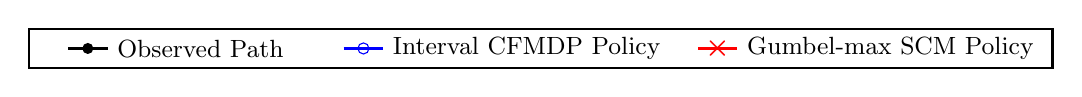
\begin{tikzpicture}[scale=1.0, every node/.style={scale=1.0}]
            \draw[thick, black] (-3, -0.25) rectangle (10, 0.25);
            %
            \draw[black, line width=1pt] (-2.5, 0.0) -- (-2,0.0);
            \fill[black] (-2.25,0.0) circle (2pt); %
            \node[right] at (-2,0.0) {\small Observed Path};
            
            %
            \draw[blue, line width=1pt] (1.0,0.0) -- (1.5,0.0);
            \node[draw=blue, circle, minimum size=4pt, inner sep=0pt] at (1.25,0.0) {}; %
            \node[right] at (1.5,0.0) {\small Interval CFMDP Policy};
            
            %
            \draw[red, line width=1pt] (5.5,0) -- (6,0);
            \node[red] at (5.75,0) {$\boldsymbol{\times}$}; %
            \node[right] at (6,0) {\small Gumbel-max SCM Policy};
        \end{tikzpicture}
    }\\
    %
    \subfigure[\footnotesize Lowest cumulative reward: Interval CFMDP ($312$), Gumbel-max SCM ($312$)]{%
        \resizebox{0.76\columnwidth}{!}{
             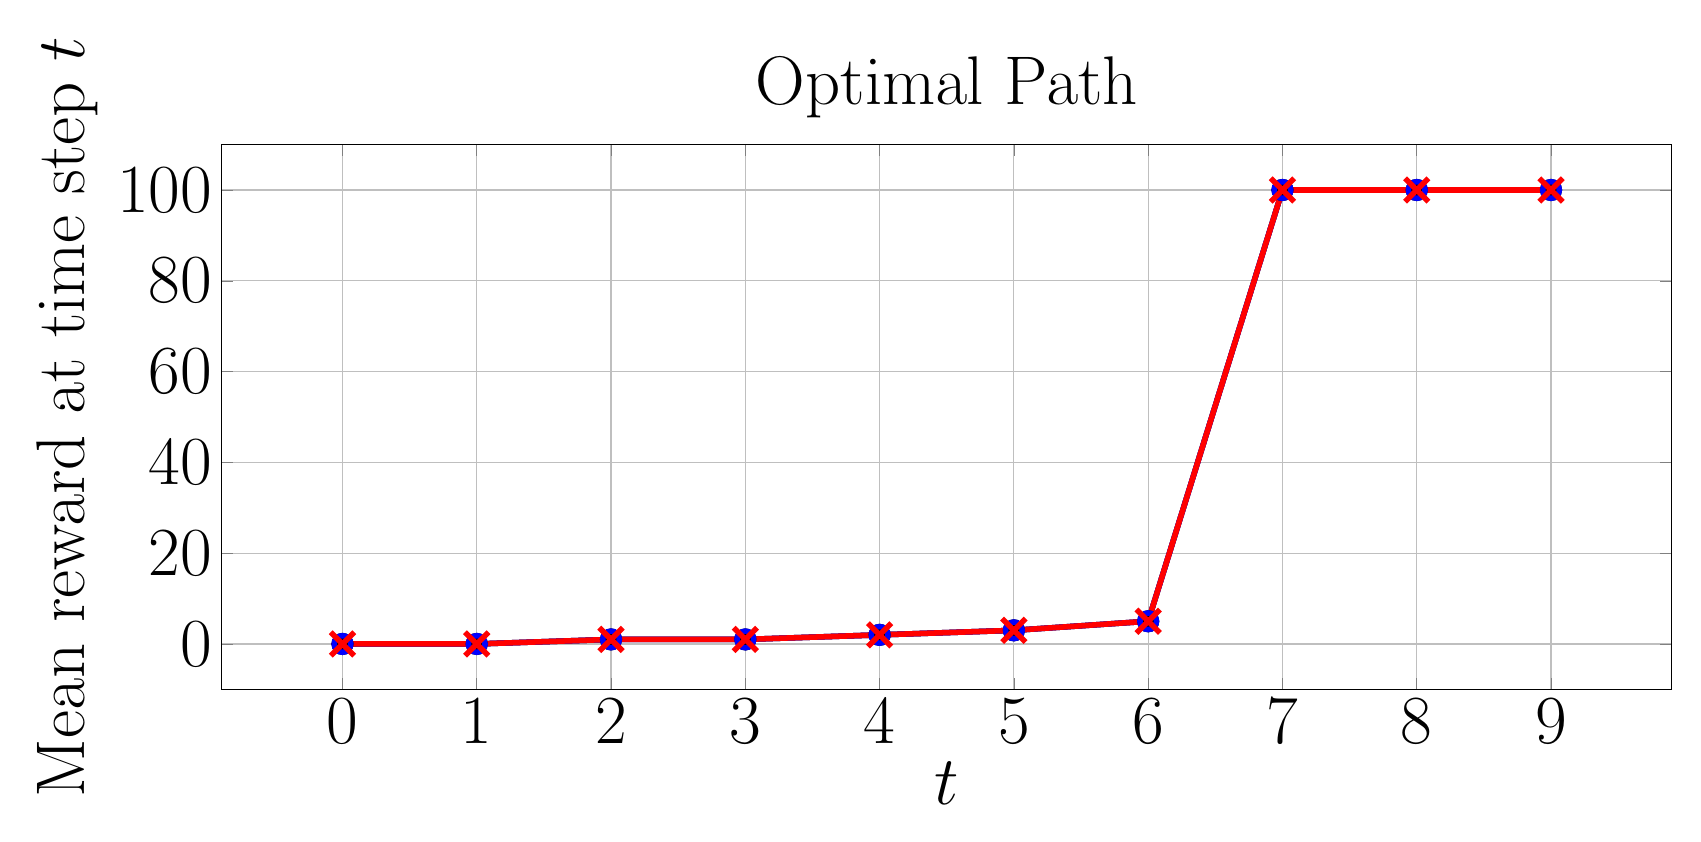
\begin{tikzpicture}
                \begin{axis}[
                    xlabel={$t$},
                    ylabel={Mean reward at time step $t$},
                    title={Optimal Path},
                    grid=both,
                    width=20cm, height=8.5cm,
                    every axis/.style={font=\Huge},
                    %
                ]
                \addplot[
                    color=black, %
                    mark=*, %
                    line width=2pt,
                    mark size=3pt,
                    error bars/.cd,
                    y dir=both, %
                    y explicit, %
                    error bar style={line width=1pt,solid},
                    error mark options={line width=1pt,mark size=4pt,rotate=90}
                ]
                coordinates {
                    (0, 0.0)  +- (0, 0.0)
                    (1, 0.0)  +- (0, 0.0) 
                    (2, 1.0)  +- (0, 0.0) 
                    (3, 1.0)  +- (0, 0.0)
                    (4, 2.0)  +- (0, 0.0)
                    (5, 3.0) +- (0, 0.0)
                    (6, 5.0) +- (0, 0.0)
                    (7, 100.0) +- (0, 0.0)
                    (8, 100.0) +- (0, 0.0)
                    (9, 100.0) +- (0, 0.0)
                };
                %
                \addplot[
                    color=blue, %
                    mark=o, %
                    line width=2pt,
                    mark size=3pt,
                    error bars/.cd,
                    y dir=both, %
                    y explicit, %
                    error bar style={line width=1pt,solid},
                    error mark options={line width=1pt,mark size=4pt,rotate=90}
                ]
                 coordinates {
                    (0, 0.0)  +- (0, 0.0)
                    (1, 0.0)  +- (0, 0.0) 
                    (2, 1.0)  +- (0, 0.0) 
                    (3, 1.0)  +- (0, 0.0)
                    (4, 2.0)  +- (0, 0.0)
                    (5, 3.0) +- (0, 0.0)
                    (6, 5.0) +- (0, 0.0)
                    (7, 100.0) +- (0, 0.0)
                    (8, 100.0) +- (0, 0.0)
                    (9, 100.0) +- (0, 0.0)
                };
                %
                \addplot[
                    color=red, %
                    mark=x, %
                    line width=2pt,
                    mark size=6pt,
                    error bars/.cd,
                    y dir=both, %
                    y explicit, %
                    error bar style={line width=1pt,solid},
                    error mark options={line width=1pt,mark size=4pt,rotate=90}
                ]
                coordinates {
                    (0, 0.0)  +- (0, 0.0)
                    (1, 0.0)  +- (0, 0.0) 
                    (2, 1.0)  +- (0, 0.0) 
                    (3, 1.0)  +- (0, 0.0)
                    (4, 2.0)  +- (0, 0.0)
                    (5, 3.0) +- (0, 0.0)
                    (6, 5.0) +- (0, 0.0)
                    (7, 100.0) +- (0, 0.0)
                    (8, 100.0) +- (0, 0.0)
                    (9, 100.0) +- (0, 0.0)
                };
                \end{axis}
            \end{tikzpicture}
         }
    }
    \hspace{1cm}
    \subfigure[\footnotesize Lowest cumulative reward: Interval CFMDP ($19$), Gumbel-max SCM ($-88$)]{%
         \resizebox{0.76\columnwidth}{!}{
            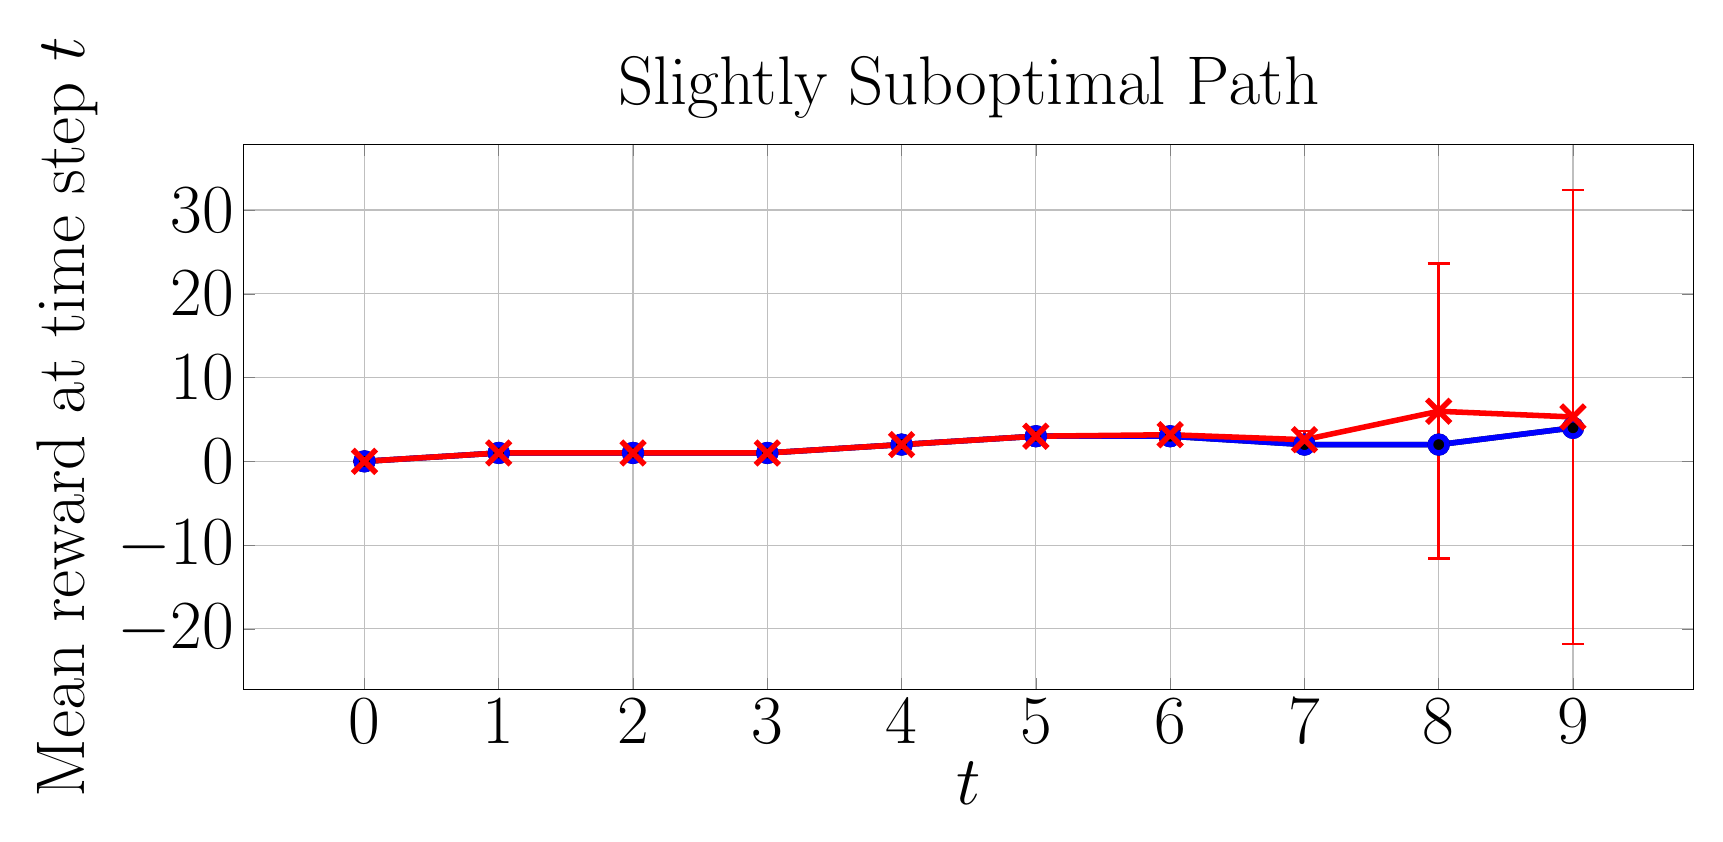
\begin{tikzpicture}
                \begin{axis}[
                    xlabel={$t$},
                    ylabel={Mean reward at time step $t$},
                    title={Slightly Suboptimal Path},
                    grid=both,
                    width=20cm, height=8.5cm,
                    every axis/.style={font=\Huge},
                    %
                ]
                \addplot[
                    color=black, %
                    mark=*, %
                    line width=2pt,
                    mark size=3pt,
                    error bars/.cd,
                    y dir=both, %
                    y explicit, %
                    error bar style={line width=1pt,solid},
                    error mark options={line width=1pt,mark size=4pt,rotate=90}
                ]
              coordinates {
                    (0, 0.0)  +- (0, 0.0)
                    (1, 1.0)  +- (0, 0.0) 
                    (2, 1.0)  +- (0, 0.0) 
                    (3, 1.0)  +- (0, 0.0)
                    (4, 2.0)  +- (0, 0.0)
                    (5, 3.0) +- (0, 0.0)
                    (6, 3.0) +- (0, 0.0)
                    (7, 2.0) +- (0, 0.0)
                    (8, 2.0) +- (0, 0.0)
                    (9, 4.0) +- (0, 0.0)
                };
                %
                \addplot[
                    color=blue, %
                    mark=o, %
                    line width=2pt,
                    mark size=3pt,
                    error bars/.cd,
                    y dir=both, %
                    y explicit, %
                    error bar style={line width=1pt,solid},
                    error mark options={line width=1pt,mark size=4pt,rotate=90}
                ]
              coordinates {
                    (0, 0.0)  +- (0, 0.0)
                    (1, 1.0)  +- (0, 0.0) 
                    (2, 1.0)  +- (0, 0.0) 
                    (3, 1.0)  +- (0, 0.0)
                    (4, 2.0)  +- (0, 0.0)
                    (5, 3.0) +- (0, 0.0)
                    (6, 3.0) +- (0, 0.0)
                    (7, 2.0) +- (0, 0.0)
                    (8, 2.0) +- (0, 0.0)
                    (9, 4.0) +- (0, 0.0)
                };
                %
                \addplot[
                    color=red, %
                    mark=x, %
                    line width=2pt,
                    mark size=6pt,
                    error bars/.cd,
                    y dir=both, %
                    y explicit, %
                    error bar style={line width=1pt,solid},
                    error mark options={line width=1pt,mark size=4pt,rotate=90}
                ]
                coordinates {
                    (0, 0.0)  +- (0, 0.0)
                    (1, 1.0)  +- (0, 0.0) 
                    (2, 1.0)  +- (0, 0.0) 
                    (3, 1.0)  +- (0, 0.0)
                    (4, 2.0)  += (0, 0.0)
                    (5, 3.0)  += (0, 0.0)
                    (6, 3.17847) += (0, 0.62606746) -= (0, 0.62606746)
                    (7, 2.5832885) += (0, 1.04598233) -= (0, 1.04598233)
                    (8, 5.978909) += (0, 17.60137623) -= (0, 17.60137623)
                    (9, 5.297059) += (0, 27.09227512) -= (0, 27.09227512)
                };
                \end{axis}
            \end{tikzpicture}
         }
    }\\[-1.5pt]
    \subfigure[\footnotesize Lowest cumulative reward: Interval CFMDP ($14$), Gumbel-max SCM ($-598$)]{%
         \resizebox{0.76\columnwidth}{!}{
             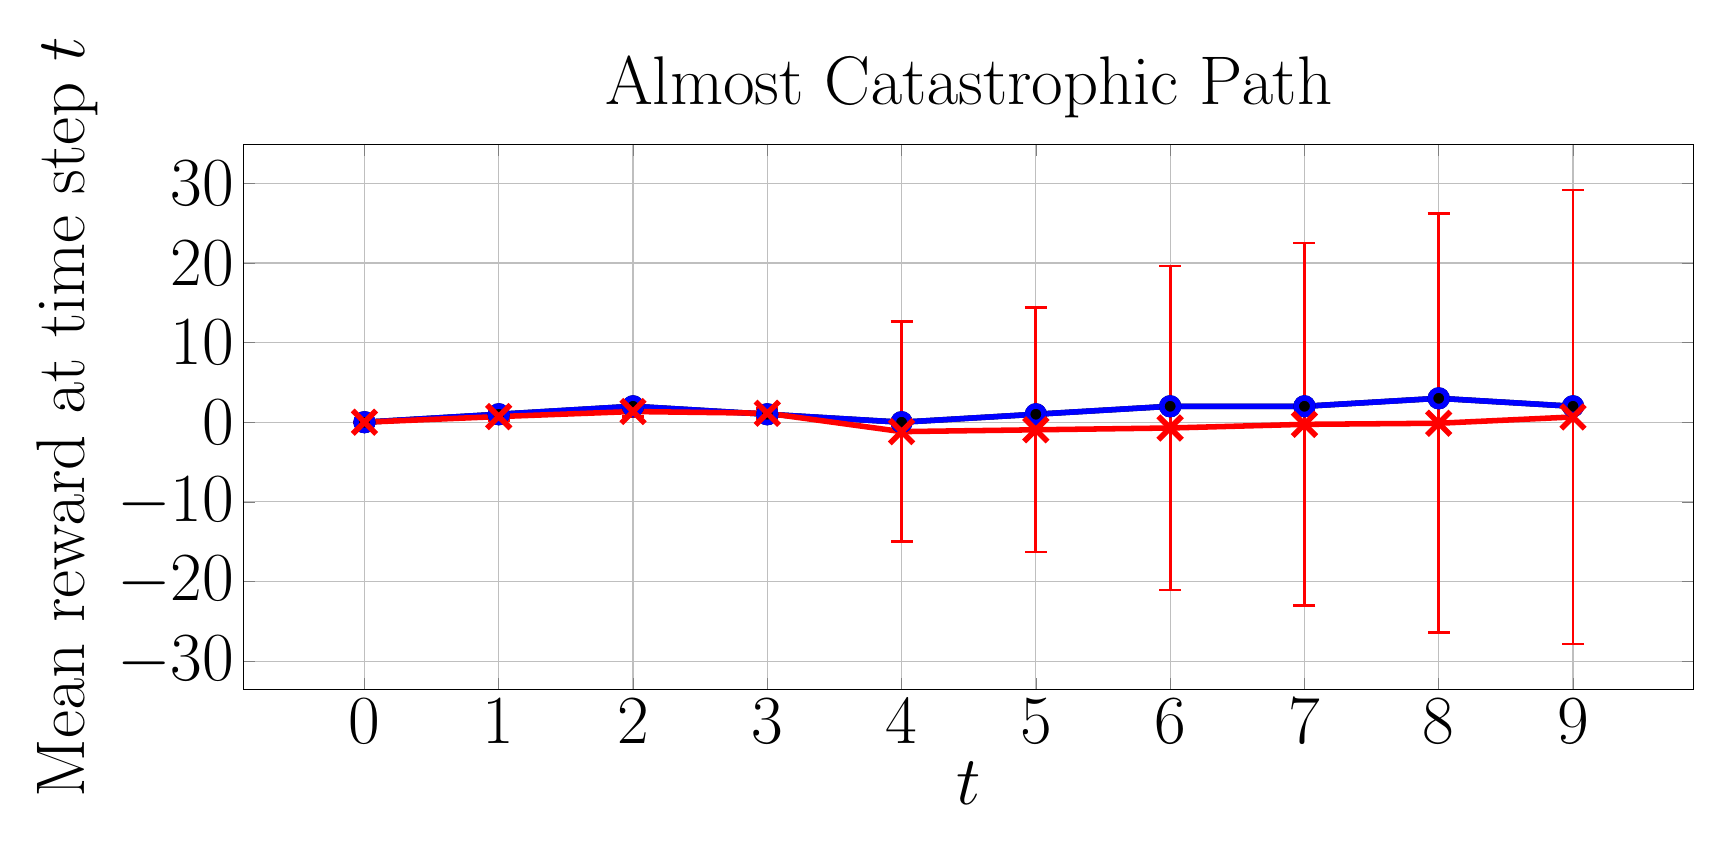
\begin{tikzpicture}
                \begin{axis}[
                    xlabel={$t$},
                    ylabel={Mean reward at time step $t$},
                    title={Almost Catastrophic Path},
                    grid=both,
                    width=20cm, height=8.5cm,
                    every axis/.style={font=\Huge},
                    %
                ]
                \addplot[
                    color=black, %
                    mark=*, %
                    line width=2pt,
                    mark size=3pt,
                    error bars/.cd,
                    y dir=both, %
                    y explicit, %
                    error bar style={line width=1pt,solid},
                    error mark options={line width=1pt,mark size=4pt,rotate=90}
                ]
                coordinates {
                    (0, 0.0)  +- (0, 0.0)
                    (1, 1.0)  +- (0, 0.0) 
                    (2, 2.0)  +- (0, 0.0) 
                    (3, 1.0)  +- (0, 0.0)
                    (4, 0.0)  +- (0, 0.0)
                    (5, 1.0) +- (0, 0.0)
                    (6, 2.0) +- (0, 0.0)
                    (7, 2.0) +- (0, 0.0)
                    (8, 3.0) +- (0, 0.0)
                    (9, 2.0) +- (0, 0.0)
                };
                %
                \addplot[
                    color=blue, %
                    mark=o, %
                    line width=2pt,
                    mark size=3pt,
                    error bars/.cd,
                    y dir=both, %
                    y explicit, %
                    error bar style={line width=1pt,solid},
                    error mark options={line width=1pt,mark size=4pt,rotate=90}
                ]
                coordinates {
                    (0, 0.0)  +- (0, 0.0)
                    (1, 1.0)  +- (0, 0.0) 
                    (2, 2.0)  +- (0, 0.0) 
                    (3, 1.0)  +- (0, 0.0)
                    (4, 0.0)  +- (0, 0.0)
                    (5, 1.0) +- (0, 0.0)
                    (6, 2.0) +- (0, 0.0)
                    (7, 2.0) +- (0, 0.0)
                    (8, 3.0) +- (0, 0.0)
                    (9, 2.0) +- (0, 0.0)
                };
                %
                \addplot[
                    color=red, %
                    mark=x, %
                    line width=2pt,
                    mark size=6pt,
                    error bars/.cd,
                    y dir=both, %
                    y explicit, %
                    error bar style={line width=1pt,solid},
                    error mark options={line width=1pt,mark size=4pt,rotate=90}
                ]
                coordinates {
                    (0, 0.0)  +- (0, 0.0)
                    (1, 0.7065655)  +- (0, 0.4553358) 
                    (2, 1.341673)  +- (0, 0.67091621) 
                    (3, 1.122926)  +- (0, 0.61281824)
                    (4, -1.1821935)  +- (0, 13.82444042)
                    (5, -0.952399)  +- (0, 15.35195457)
                    (6, -0.72672) +- (0, 20.33508414)
                    (7, -0.268983) +- (0, 22.77861454)
                    (8, -0.1310835) +- (0, 26.31013314)
                    (9, 0.65806) +- (0, 28.50670214)
                };
                %
            %
            %
            %
            %
            %
            %
            %
            %
            %
            %
            %
            %
            %
            %
            %
            %
            %
            %
                \end{axis}
            \end{tikzpicture}
         }
    }
    \hspace{1cm}
    \subfigure[\footnotesize Lowest cumulative reward: Interval CFMDP ($-698$), Gumbel-max SCM ($-698$)]{%
         \resizebox{0.76\columnwidth}{!}{
            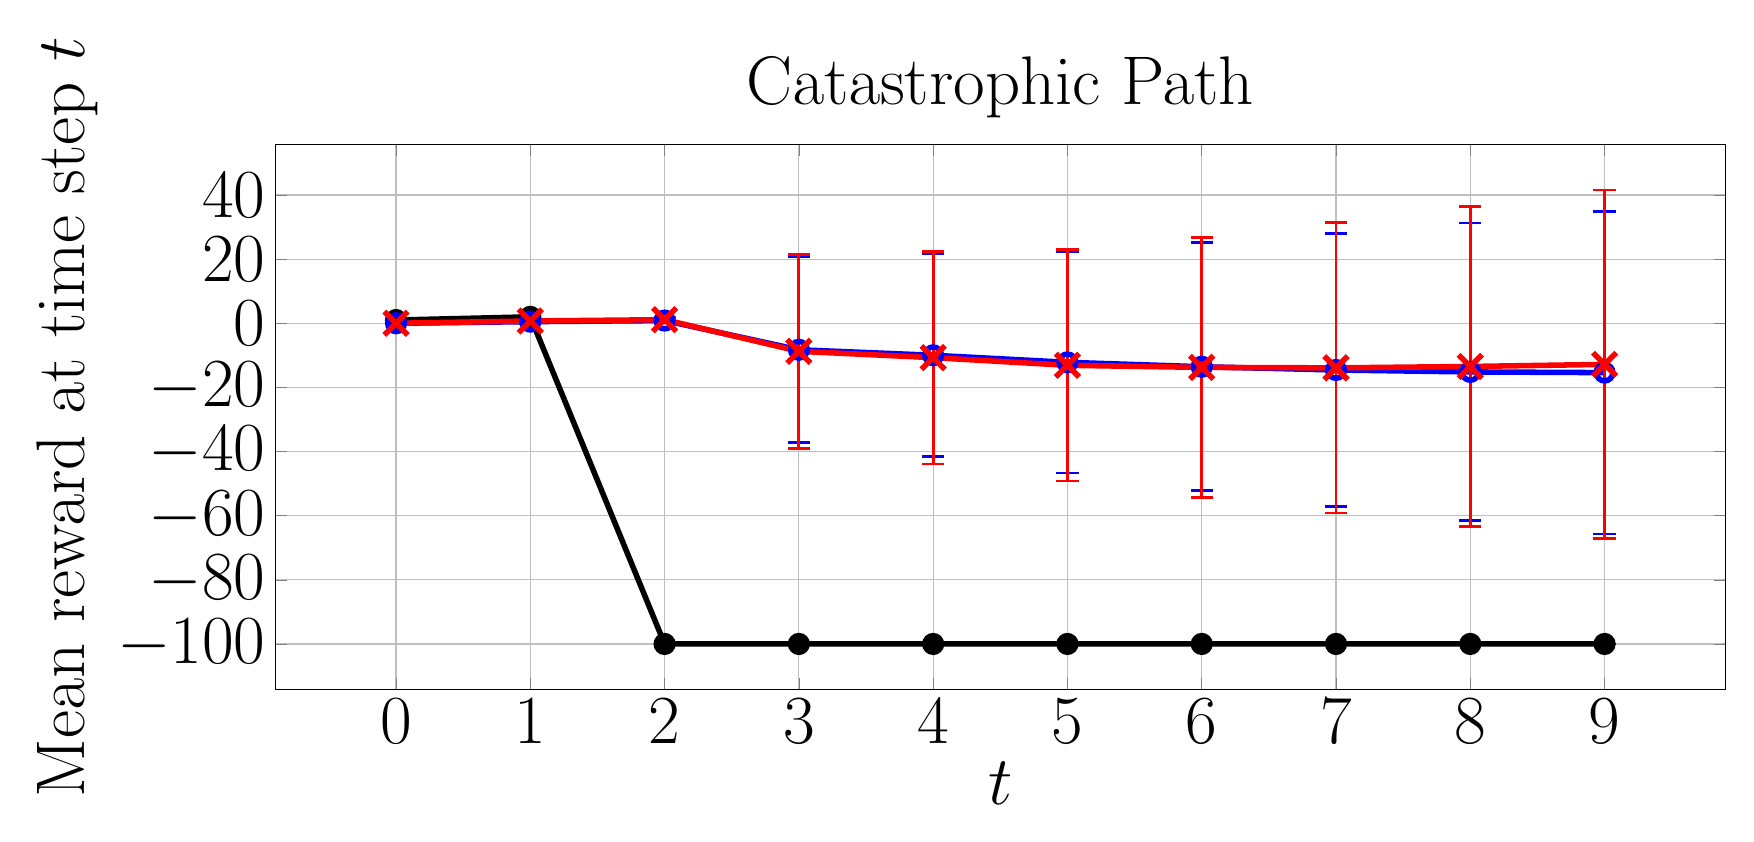
\begin{tikzpicture}
                \begin{axis}[
                    xlabel={$t$},
                    ylabel={Mean reward at time step $t$},
                    title={Catastrophic Path},
                    grid=both,
                    width=20cm, height=8.5cm,
                    every axis/.style={font=\Huge},
                    %
                ]
                \addplot[
                    color=black, %
                    mark=*, %
                    line width=2pt,
                    mark size=3pt,
                    error bars/.cd,
                    y dir=both, %
                    y explicit, %
                    error bar style={line width=1pt,solid},
                    error mark options={line width=1pt,mark size=4pt,rotate=90}
                ]
                coordinates {
                    (0, 1.0)  +- (0, 0.0)
                    (1, 2.0)  +- (0, 0.0) 
                    (2, -100.0)  +- (0, 0.0) 
                    (3, -100.0)  +- (0, 0.0)
                    (4, -100.0)  +- (0, 0.0)
                    (5, -100.0) +- (0, 0.0)
                    (6, -100.0) +- (0, 0.0)
                    (7, -100.0) +- (0, 0.0)
                    (8, -100.0) +- (0, 0.0)
                    (9, -100.0) +- (0, 0.0)
                };
                %
                \addplot[
                    color=blue, %
                    mark=o, %
                    line width=2pt,
                    mark size=3pt,
                    error bars/.cd,
                    y dir=both, %
                    y explicit, %
                    error bar style={line width=1pt,solid},
                    error mark options={line width=1pt,mark size=4pt,rotate=90}
                ]
                coordinates {
                    (0, 0.0)  +- (0, 0.0)
                    (1, 0.504814)  +- (0, 0.49997682) 
                    (2, 0.8439835)  +- (0, 0.76831917) 
                    (3, -8.2709165)  +- (0, 28.93656754)
                    (4, -9.981082)  +- (0, 31.66825363)
                    (5, -12.1776325) +- (0, 34.53463233)
                    (6, -13.556076) +- (0, 38.62845372)
                    (7, -14.574418) +- (0, 42.49603359)
                    (8, -15.1757075) +- (0, 46.41913968)
                    (9, -15.3900395) +- (0, 50.33563368)
                };
                %
                \addplot[
                    color=red, %
                    mark=x, %
                    line width=2pt,
                    mark size=6pt,
                    error bars/.cd,
                    y dir=both, %
                    y explicit, %
                    error bar style={line width=1pt,solid},
                    error mark options={line width=1pt,mark size=4pt,rotate=90}
                ]
                coordinates {
                    (0, 0.0)  +- (0, 0.0)
                    (1, 0.701873)  +- (0, 0.45743556) 
                    (2, 1.1227805)  +- (0, 0.73433129) 
                    (3, -8.7503255)  +- (0, 30.30257976)
                    (4, -10.722092)  +- (0, 33.17618589)
                    (5, -13.10721)  +- (0, 36.0648089)
                    (6, -13.7631645) +- (0, 40.56553451)
                    (7, -13.909043) +- (0, 45.23829402)
                    (8, -13.472517) +- (0, 49.96270296)
                    (9, -12.8278835) +- (0, 54.38618735)
                };
                %
            %
            %
            %
            %
            %
            %
            %
            %
            %
            %
            %
            %
            %
            %
            %
            %
            %
            %
                \end{axis}
            \end{tikzpicture}
         }
    }
    \caption{Average instant reward of CF paths induced by policies on GridWorld $p=0.4$.}
    \label{fig: reward p=0.4}
\end{figure*}

\subsection{Experimental Setup}
To compare policy performance, we measure the average rewards of counterfactual paths induced by our policy and the Gumbel-max policy by uniformly sampling $200$ counterfactual MDPs from the ICFMDP and generating $10,000$ counterfactual paths over each sampled CFMDP. \jl{Since the interval CFMDP depends on the observed path, we select $4$  paths of varying optimality to evaluate how the observed path impacts the performance of both policies: an optimal path, a slightly suboptimal path that could reach the optimal reward with a few changes, a catastrophic path that enters a catastrophic, terminal state with low reward, and an almost catastrophic path that was close to entering a catastrophic state.} When measuring the average probability bound widths and execution time needed to generate the ICFMDPs, we averaged over $20$ randomly generated observed paths
\footnote{Further training details are provided in Appendix \ref{app: training details}, and the code is provided at \href{https://github.com/ddv-lab/robust-cf-inference-in-MDPs}{https://github.com/ddv-lab/robust-cf-inference-in-MDPs}
%
%
.}.

\subsection{GridWorld}
\jl{The GridWorld MDP is a $4 \times 4$ grid where an agent must navigate from the top-left corner to the goal state in the bottom-right corner, avoiding a dangerous terminal state in the centre. At each time step, the agent can move up, down, left, or right, but there is a small probability (controlled by hyper-parameter $p$) of moving in an unintended direction. As the agent nears the goal, the reward for each state increases, culminating in a reward of $+100$ for reaching the goal. Entering the dangerous state results in a penalty of $-100$. We use two versions of GridWorld: a less stochastic version with $p=0.9$ (i.e., $90$\% chance of moving in the chosen direction) and a more stochastic version with $p=0.4$.}

\paragraph{GridWorld ($p=0.9$)}
When $p=0.9$, the counterfactual probability bounds are typically narrow (see Table \ref{tab:nonzero_probs} for average measurements). Consequently, as shown in Figure \ref{fig: reward p=0.9}, both policies are nearly identical and perform similarly well across the optimal, slightly suboptimal, and catastrophic paths.
%
However, for the almost catastrophic path, the interval CFMDP path is more conservative and follows the observed path more closely (as this is where the probability bounds are narrowest), which typically requires one additional step to reach the goal state than the Gumbel-max SCM policy.
%

\paragraph{GridWorld ($p=0.4$)}
\jl{When $p=0.4$, the GridWorld environment becomes more uncertain, increasing the risk of entering the dangerous state even if correct actions are chosen. Thus, as shown in Figure \ref{fig: reward p=0.4}, the interval CFMDP policy adopts a more conservative approach, avoiding deviation from the observed policy if it cannot guarantee higher counterfactual rewards (see the slightly suboptimal and almost catastrophic paths), whereas the Gumbel-max SCM is inconsistent: it can yield higher rewards, but also much lower rewards, reflected in the wide error bars.} For the catastrophic path, both policies must deviate from the observed path to achieve a higher reward and, in this case, perform similarly.
%
%
%
%
\subsection{Sepsis}
The Sepsis MDP \citep{oberst2019counterfactual} simulates trajectories of Sepsis patients. Each state consists of four vital signs (heart rate, blood pressure, oxygen concentration, and glucose levels), categorised as low, normal, or high.
and three treatments that can be toggled on/off at each time step (8 actions in total). Unlike \citet{oberst2019counterfactual}, we scale rewards based on the number of out-of-range vital signs, between $-1000$ (patient dies) and $1000$ (patient discharged). \jl{Like the GridWorld $p=0.4$ experiment, the Sepsis MDP is highly uncertain, as many states are equally likely to lead to optimal and poor outcomes. Thus, as shown in Figure \ref{fig: reward sepsis}, both policies follow the observed optimal and almost catastrophic paths to guarantee rewards are no worse than the observation.} However, improving the catastrophic path requires deviating from the observation. Here, the Gumbel-max SCM policy, on average, performs better than the interval CFMDP policy. But, since both policies have lower bounds clipped at $-1000$, neither policy reliably improves over the observation. In contrast, for the slightly suboptimal path, the interval CFMDP policy performs significantly better, shown by its higher lower bounds. 
Moreover, in these two cases, the worst-case counterfactual path generated by the interval CFMDP policy is better than that of the Gumbel-max SCM policy,
indicating its greater robustness.
%
\begin{figure*}
    \centering
     \resizebox{0.6\textwidth}{!}{
        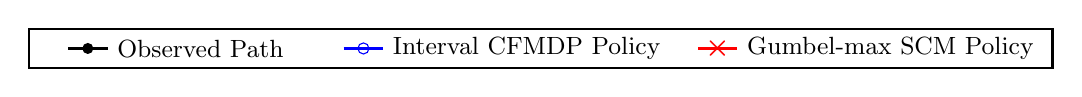
\begin{tikzpicture}[scale=1.0, every node/.style={scale=1.0}]
            \draw[thick, black] (-3, -0.25) rectangle (10, 0.25);
            %
            \draw[black, line width=1pt] (-2.5, 0.0) -- (-2,0.0);
            \fill[black] (-2.25,0.0) circle (2pt); %
            \node[right] at (-2,0.0) {\small Observed Path};
            
            %
            \draw[blue, line width=1pt] (1.0,0.0) -- (1.5,0.0);
            \node[draw=blue, circle, minimum size=4pt, inner sep=0pt] at (1.25,0.0) {}; %
            \node[right] at (1.5,0.0) {\small Interval CFMDP Policy};
            
            %
            \draw[red, line width=1pt] (5.5,0) -- (6,0);
            \node[red] at (5.75,0) {$\boldsymbol{\times}$}; %
            \node[right] at (6,0) {\small Gumbel-max SCM Policy};
        \end{tikzpicture}
    }\\
    \subfigure[\footnotesize Lowest cumulative reward: Interval CFMDP ($8000$), Gumbel-max SCM ($8000$)]{%
         \resizebox{0.76\columnwidth}{!}{
             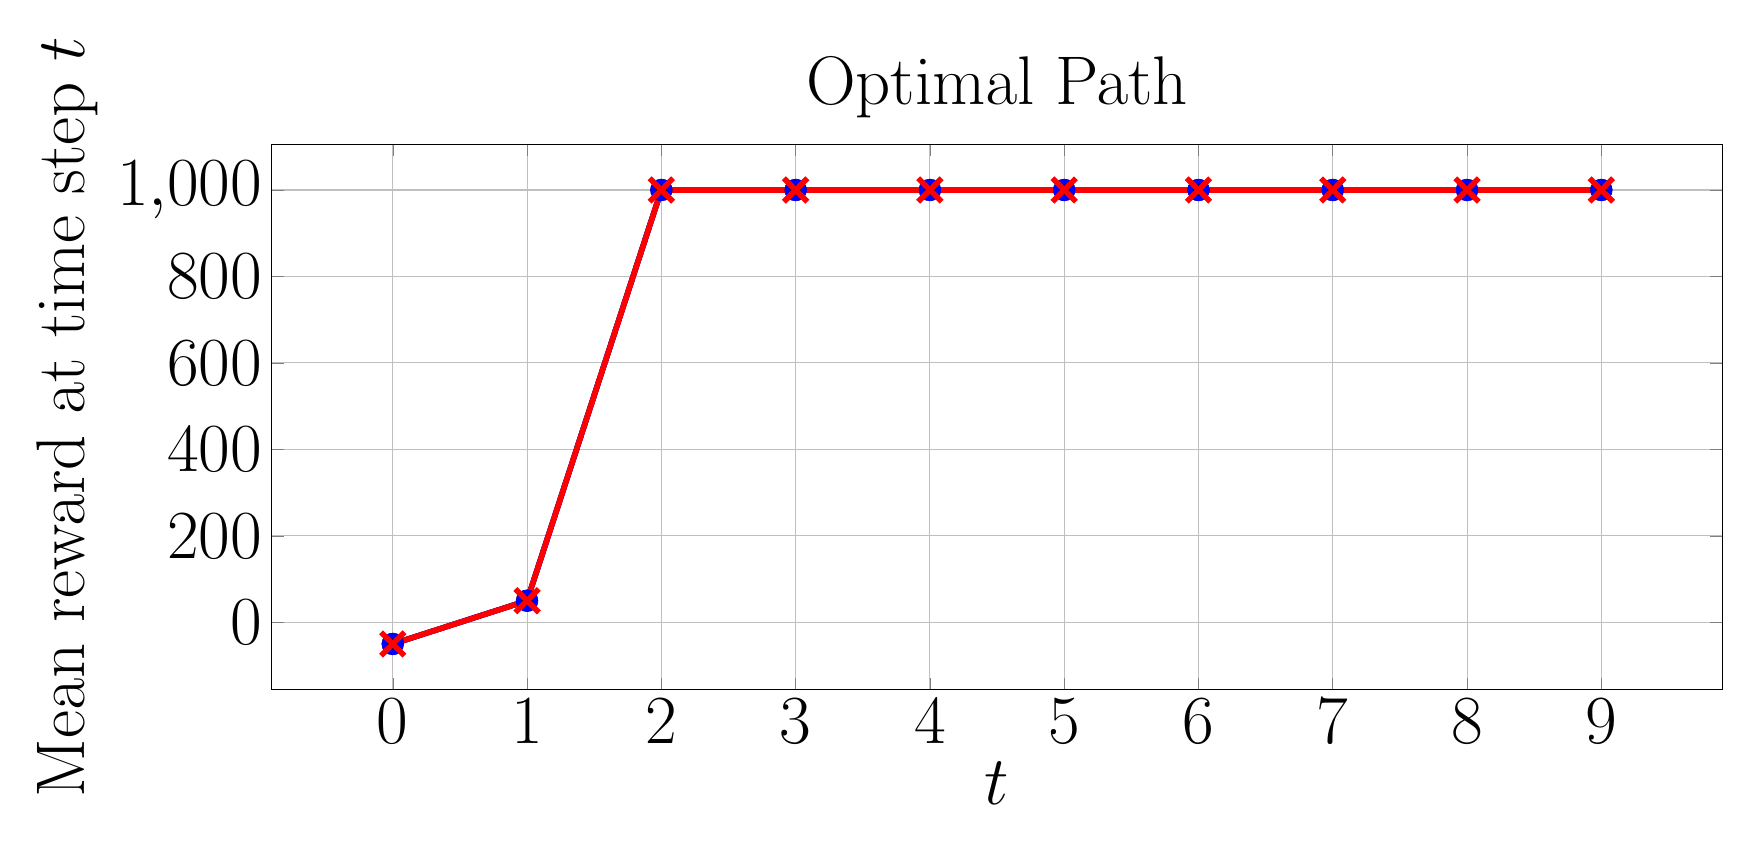
\begin{tikzpicture}
                \begin{axis}[
                    xlabel={$t$},
                    ylabel={Mean reward at time step $t$},
                    title={Optimal Path},
                    grid=both,
                    width=20cm, height=8.5cm,
                    every axis/.style={font=\Huge},
                    %
                ]
                \addplot[
                    color=black, %
                    mark=*, %
                    line width=2pt,
                    mark size=3pt,
                ]
                coordinates {
                    (0, -50.0)
                    (1, 50.0)
                    (2, 1000.0)
                    (3, 1000.0)
                    (4, 1000.0)
                    (5, 1000.0)
                    (6, 1000.0)
                    (7, 1000.0)
                    (8, 1000.0)
                    (9, 1000.0)
                };
                %
                \addplot[
                    color=blue, %
                    mark=o, %
                    line width=2pt,
                    mark size=3pt,
                    error bars/.cd,
                    y dir=both, %
                    y explicit, %
                    error bar style={line width=1pt,solid},
                    error mark options={line width=1pt,mark size=4pt,rotate=90}
                ]
                coordinates {
                    (0, -50.0)  +- (0, 0.0)
                    (1, 50.0)  +- (0, 0.0) 
                    (2, 1000.0)  +- (0, 0.0) 
                    (3, 1000.0)  +- (0, 0.0)
                    (4, 1000.0)  +- (0, 0.0)
                    (5, 1000.0) +- (0, 0.0)
                    (6, 1000.0) +- (0, 0.0)
                    (7, 1000.0) +- (0, 0.0)
                    (8, 1000.0) +- (0, 0.0)
                    (9, 1000.0) +- (0, 0.0)
                };
                %
                \addplot[
                    color=red, %
                    mark=x, %
                    line width=2pt,
                    mark size=6pt,
                    error bars/.cd,
                    y dir=both, %
                    y explicit, %
                    error bar style={line width=1pt,solid},
                    error mark options={line width=1pt,mark size=4pt,rotate=90}
                ]
                coordinates {
                    (0, -50.0)  +- (0, 0.0)
                    (1, 50.0)  +- (0, 0.0) 
                    (2, 1000.0)  +- (0, 0.0) 
                    (3, 1000.0)  +- (0, 0.0)
                    (4, 1000.0)  +- (0, 0.0)
                    (5, 1000.0) +- (0, 0.0)
                    (6, 1000.0) +- (0, 0.0)
                    (7, 1000.0) +- (0, 0.0)
                    (8, 1000.0) +- (0, 0.0)
                    (9, 1000.0) +- (0, 0.0)
                };
                %
                \end{axis}
            \end{tikzpicture}
         }
    }
    \hspace{1cm}
    \subfigure[\footnotesize Lowest cumulative reward: Interval CFMDP ($-5980$), Gumbel-max SCM ($-8000$)]{%
         \resizebox{0.76\columnwidth}{!}{
            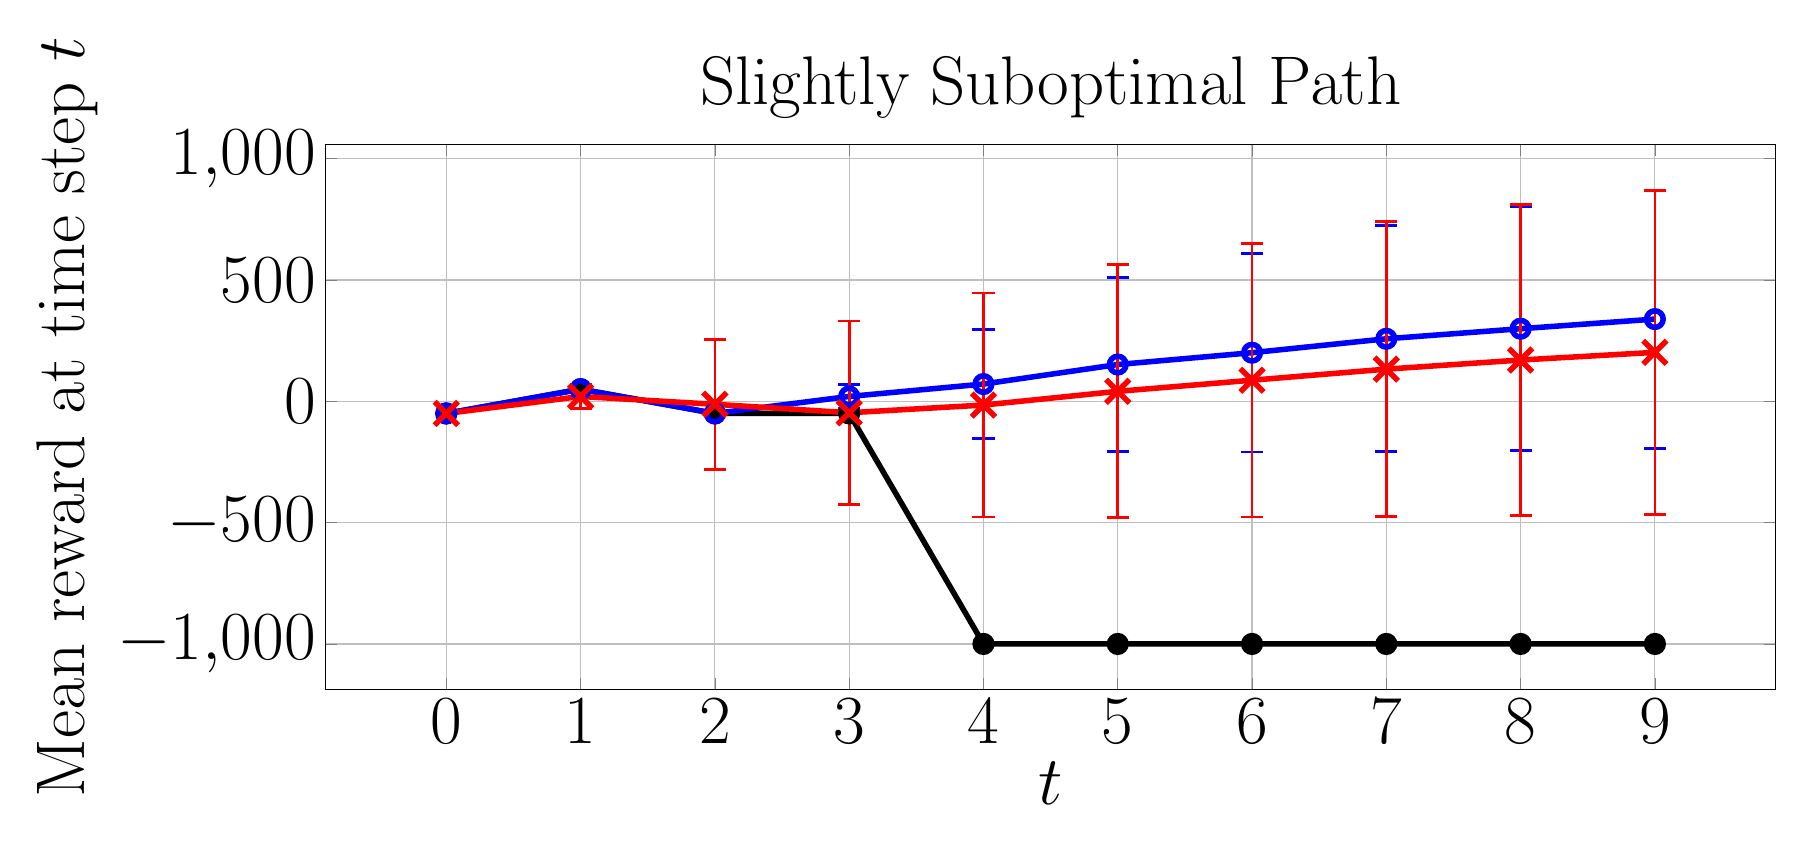
\begin{tikzpicture}
                \begin{axis}[
                    xlabel={$t$},
                    ylabel={Mean reward at time step $t$},
                    title={Slightly Suboptimal Path},
                    grid=both,
                    width=20cm, height=8.5cm,
                    every axis/.style={font=\Huge},
                    %
                ]
               \addplot[
                    color=black, %
                    mark=*, %
                    line width=2pt,
                    mark size=3pt,
                ]
                coordinates {
                    (0, -50.0)
                    (1, 50.0)
                    (2, -50.0)
                    (3, -50.0)
                    (4, -1000.0)
                    (5, -1000.0)
                    (6, -1000.0)
                    (7, -1000.0)
                    (8, -1000.0)
                    (9, -1000.0)
                };
                %
                \addplot[
                    color=blue, %
                    mark=o, %
                    line width=2pt,
                    mark size=3pt,
                    error bars/.cd,
                    y dir=both, %
                    y explicit, %
                    error bar style={line width=1pt,solid},
                    error mark options={line width=1pt,mark size=4pt,rotate=90}
                ]
                coordinates {
                    (0, -50.0)  +- (0, 0.0)
                    (1, 50.0)  +- (0, 0.0) 
                    (2, -50.0)  +- (0, 0.0) 
                    (3, 20.0631)  +- (0, 49.97539413)
                    (4, 71.206585)  +- (0, 226.02033693)
                    (5, 151.60797) +- (0, 359.23292559)
                    (6, 200.40593) +- (0, 408.86185176)
                    (7, 257.77948) +- (0, 466.10372804)
                    (8, 299.237465) +- (0, 501.82579506)
                    (9, 338.9129) +- (0, 532.06124996)
                };
                %
                \addplot[
                    color=red, %
                    mark=x, %
                    line width=2pt,
                    mark size=6pt,
                    error bars/.cd,
                    y dir=both, %
                    y explicit, %
                    error bar style={line width=1pt,solid},
                    error mark options={line width=1pt,mark size=4pt,rotate=90}
                ]
                coordinates {
                    (0, -50.0)  +- (0, 0.0)
                    (1, 20.00736)  +- (0, 49.99786741) 
                    (2, -12.282865)  +- (0, 267.598755) 
                    (3, -47.125995)  +- (0, 378.41755832)
                    (4, -15.381965)  +- (0, 461.77616558)
                    (5, 41.15459) +- (0, 521.53189262)
                    (6, 87.01595) +- (0, 564.22243126 )
                    (7, 132.62376) +- (0, 607.31338037)
                    (8, 170.168145) +- (0, 641.48013693)
                    (9, 201.813135) +- (0, 667.29441777)
                };
                %
                %
                %
                %
                %
                %
                %
                %
                %
                %
                %
                %
                %
                %
                %
                %
                %
                %
                %
                \end{axis}
            \end{tikzpicture}
         }
    }\\[-1.5pt]
    \subfigure[\footnotesize Lowest cumulative reward: Interval CFMDP ($100$), Gumbel-max SCM ($100$)]{%
         \resizebox{0.76\columnwidth}{!}{
             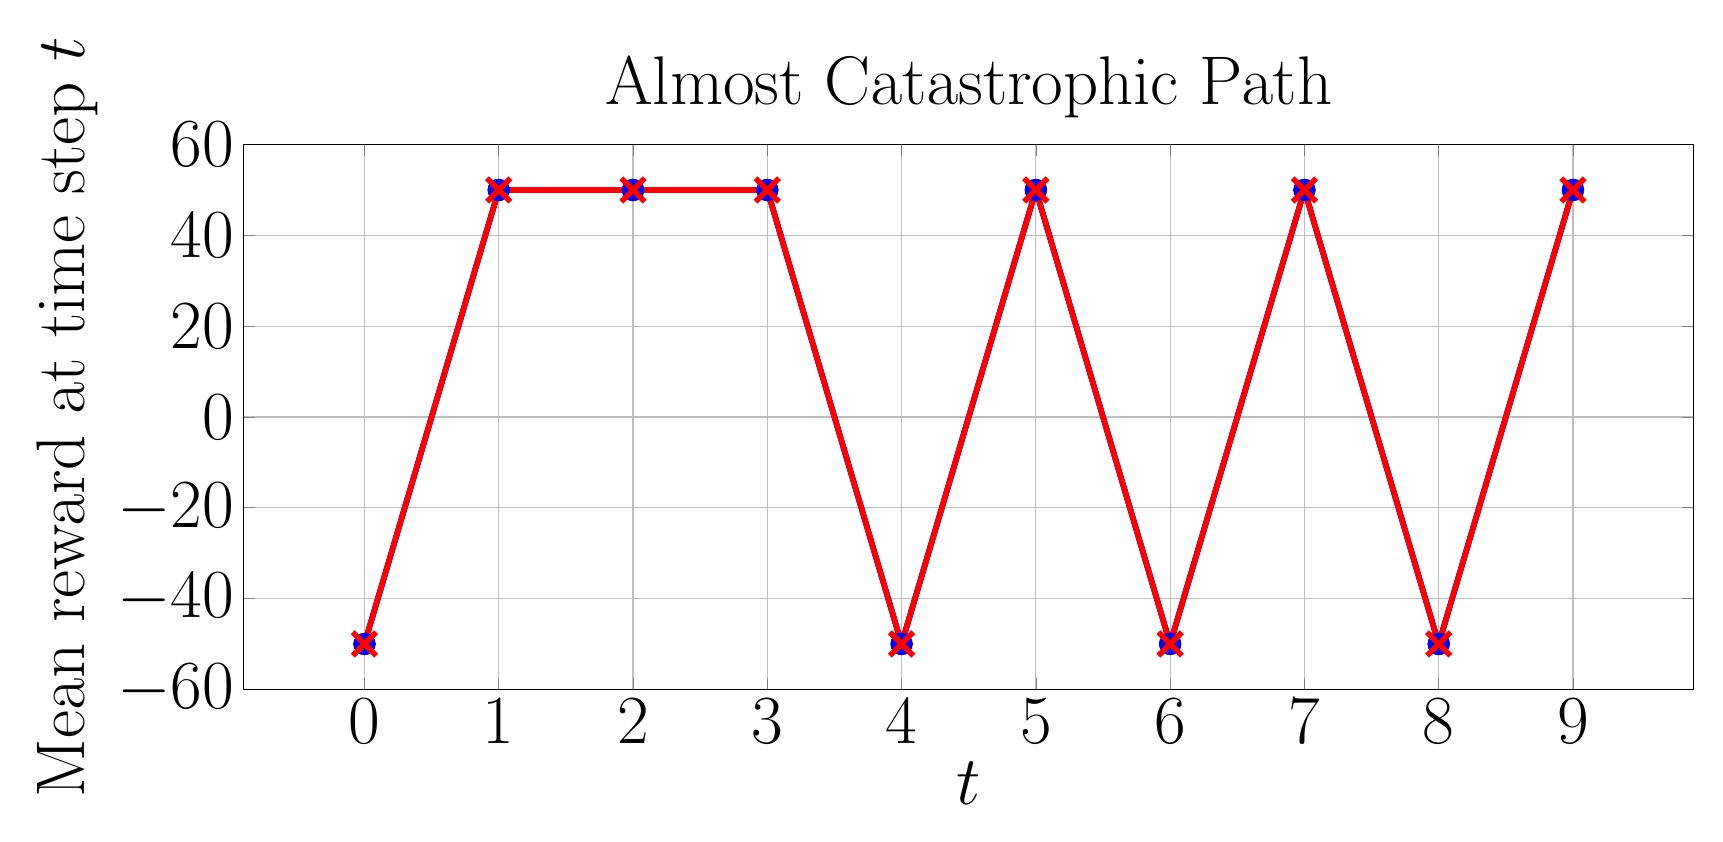
\begin{tikzpicture}
                \begin{axis}[
                    xlabel={$t$},
                    ylabel={Mean reward at time step $t$},
                    title={Almost Catastrophic Path},
                    grid=both,
                    every axis/.style={font=\Huge},
                    width=20cm, height=8.5cm,
                    %
                ]
               \addplot[
                    color=black, %
                    mark=*, %
                    line width=2pt,
                    mark size=3pt,
                ]
                coordinates {
                    (0, -50.0)
                    (1, 50.0)
                    (2, 50.0)
                    (3, 50.0)
                    (4, -50.0)
                    (5, 50.0)
                    (6, -50.0)
                    (7, 50.0)
                    (8, -50.0)
                    (9, 50.0)
                };
                %
                %
                \addplot[
                    color=blue, %
                    mark=o, %
                    line width=2pt,
                    mark size=3pt,
                    error bars/.cd,
                    y dir=both, %
                    y explicit, %
                    error bar style={line width=1pt,solid},
                    error mark options={line width=1pt,mark size=4pt,rotate=90}
                ]
                coordinates {
                    (0, -50.0)  +- (0, 0.0)
                    (1, 50.0)  +- (0, 0.0) 
                    (2, 50.0)  +- (0, 0.0) 
                    (3, 50.0)  +- (0, 0.0)
                    (4, -50.0)  +- (0, 0.0)
                    (5, 50.0) +- (0, 0.0)
                    (6, -50.0) +- (0, 0.0)
                    (7, 50.0) +- (0, 0.0)
                    (8, -50.0) +- (0, 0.0)
                    (9, 50.0) +- (0, 0.0)
                };
                %
                \addplot[
                    color=red, %
                    mark=x, %
                    line width=2pt,
                    mark size=6pt,
                    error bars/.cd,
                    y dir=both, %
                    y explicit, %
                    error bar style={line width=1pt,solid},
                    error mark options={line width=1pt,mark size=4pt,rotate=90}
                ]
                coordinates {
                    (0, -50.0)  +- (0, 0.0)
                    (1, 50.0)  +- (0, 0.0) 
                    (2, 50.0)  +- (0, 0.0) 
                    (3, 50.0)  +- (0, 0.0)
                    (4, -50.0)  +- (0, 0.0)
                    (5, 50.0) +- (0, 0.0)
                    (6, -50.0) +- (0, 0.0)
                    (7, 50.0) +- (0, 0.0)
                    (8, -50.0) +- (0, 0.0)
                    (9, 50.0) +- (0, 0.0)
                };
                %
                %
                %
                %
                %
                %
                %
                %
                %
                %
                %
                %
                %
                %
                %
                %
                %
                %
                %
                \end{axis}
            \end{tikzpicture}
         }
    }
    \hspace{1cm}
    \subfigure[\footnotesize Lowest cumulative reward: Interval CFMDP ($-7150$), Gumbel-max SCM ($-9050$)]{%
         \resizebox{0.76\columnwidth}{!}{
            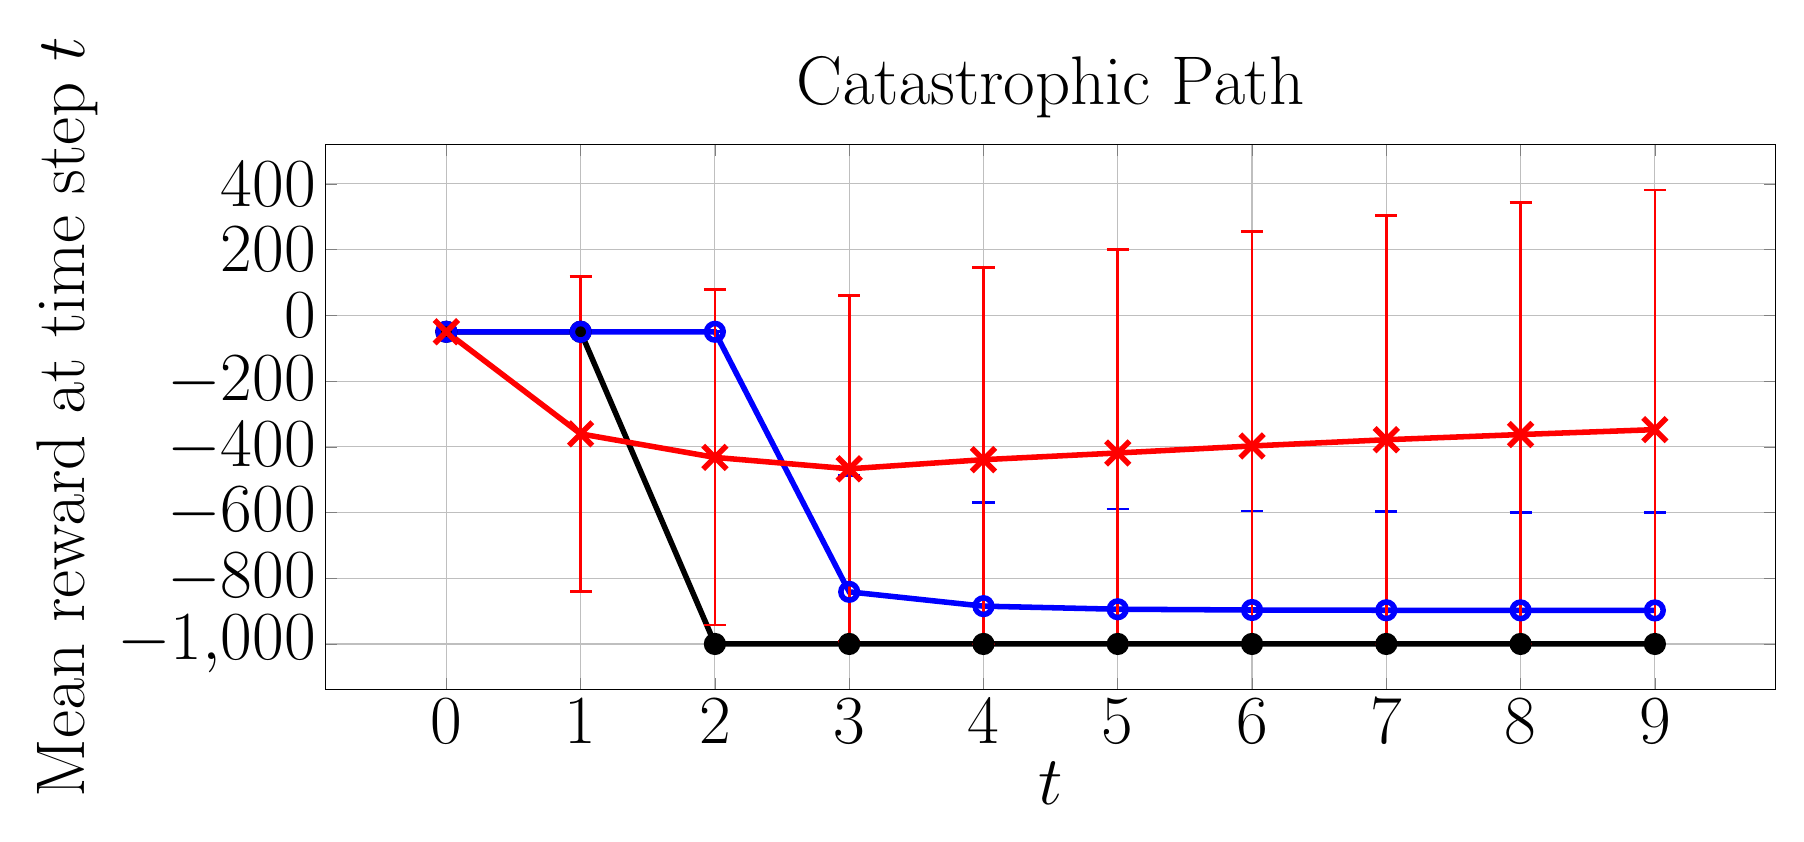
\begin{tikzpicture}
                \begin{axis}[
                    xlabel={$t$},
                    ylabel={Mean reward at time step $t$},
                    title={Catastrophic Path},
                    grid=both,
                    width=20cm, height=8.5cm,
                    every axis/.style={font=\Huge},
                    %
                ]
               \addplot[
                    color=black, %
                    mark=*, %
                    line width=2pt,
                    mark size=3pt,
                ]
                coordinates {
                    (0, -50.0)
                    (1, -50.0)
                    (2, -1000.0)
                    (3, -1000.0)
                    (4, -1000.0)
                    (5, -1000.0)
                    (6, -1000.0)
                    (7, -1000.0)
                    (8, -1000.0)
                    (9, -1000.0)
                };
                %
                %
                \addplot[
                    color=blue, %
                    mark=o, %
                    line width=2pt,
                    mark size=3pt,
                    error bars/.cd,
                    y dir=both, %
                    y explicit, %
                    error bar style={line width=1pt,solid},
                    error mark options={line width=1pt,mark size=4pt,rotate=90}
                ]
                coordinates {
                    (0, -50.0)  +- (0, 0.0)
                    (1, -50.0)  +- (0, 0.0) 
                    (2, -50.0)  +- (0, 0.0) 
                    (3, -841.440725)  += (0, 354.24605512) -= (0, 158.559275)
                    (4, -884.98225)  += (0, 315.37519669) -= (0, 115.01775)
                    (5, -894.330425) += (0, 304.88572805) -= (0, 105.669575)
                    (6, -896.696175) += (0, 301.19954514) -= (0, 103.303825)
                    (7, -897.4635) += (0, 299.61791279) -= (0, 102.5365)
                    (8, -897.77595) += (0, 298.80392585) -= (0, 102.22405)
                    (9, -897.942975) += (0, 298.32920557) -= (0, 102.057025)
                };
                %
                \addplot[
                    color=red, %
                    mark=x, %
                    line width=2pt,
                    mark size=6pt,
                    error bars/.cd,
                    y dir=both, %
                    y explicit, %
                    error bar style={line width=1pt,solid},
                    error mark options={line width=1pt,mark size=4pt,rotate=90}
                ]
            coordinates {
                    (0, -50.0)  +- (0, 0.0)
                    (1, -360.675265)  +- (0, 479.39812699) 
                    (2, -432.27629)  +- (0, 510.38620897) 
                    (3, -467.029545)  += (0, 526.36009628) -= (0, 526.36009628)
                    (4, -439.17429)  += (0, 583.96638919) -= (0, 560.82571)
                    (5, -418.82704) += (0, 618.43027478) -= (0, 581.17296)
                    (6, -397.464895) += (0, 652.67322574) -= (0, 602.535105)
                    (7, -378.49052) += (0, 682.85407033) -= (0, 621.50948)
                    (8, -362.654195) += (0, 707.01412023) -= (0, 637.345805)
                    (9, -347.737935) += (0, 729.29076479) -= (0, 652.262065)
                };
                %
                %
                %
                %
                %
                %
                %
                %
                %
                %
                %
                %
                %
                %
                %
                %
                %
                %
                %
                \end{axis}
            \end{tikzpicture}
         }
    }
    \caption{Average instant reward of CF paths induced by policies on Sepsis.}
    \label{fig: reward sepsis}
\end{figure*}

%
%
%
\subsection{Interval CFMDP Bounds}
%
%
Table \ref{tab:nonzero_probs} presents the mean counterfactual probability bound widths (excluding transitions where the upper bound is $0$) for each MDP, averaged over 20 observed paths. We compare the bounds under counterfactual stability (CS) and monotonicity (M) assumptions, CS alone, and no assumptions. This shows that the assumptions marginally reduce the bound widths, indicating the assumptions tighten the bounds without excluding too many causal models, as intended.
\renewcommand{\arraystretch}{1}

\begin{table}
\centering
\caption{Mean width of counterfactual probability bounds}
\resizebox{0.8\columnwidth}{!}{%
\begin{tabular}{|c|c|c|c|}
\hline
\multirow{2}{*}{\textbf{Environment}} & \multicolumn{3}{c|}{\textbf{Assumptions}} \\ \cline{2-4}
 & \textbf{CS + M} & \textbf{CS} & \textbf{None\tablefootnote{\jl{Equivalent to \citet{li2024probabilities}'s bounds (see Section \ref{sec: equivalence with Li}).}}} \\ \hline
\textbf{GridWorld} ($p=0.9$) & 0.0817 & 0.0977 & 0.100 \\ \hline
\textbf{GridWorld} ($p=0.4$) & 0.552  & 0.638  & 0.646 \\ \hline
\textbf{Sepsis} & 0.138 & 0.140 & 0.140 \\ \hline
\end{tabular}
}
\label{tab:nonzero_probs}
\end{table}


\subsection{Execution Times}
Table \ref{tab: times} compares the average time needed to generate the interval CFMDP vs.\ the Gumbel-max SCM CFMDP for 20 observations.
The GridWorld algorithms were run single-threaded, while the Sepsis experiments were run in parallel.
Generating the interval CFMDP is significantly faster as it uses exact analytical bounds, whereas the Gumbel-max CFMDP requires sampling from the Gumbel distribution to estimate counterfactual transition probabilities. \jl{Since constructing the counterfactual MDP models is the main bottleneck in both approaches, ours is more efficient overall and suitable for larger MDPs.}
\begin{table}
\centering
\caption{Mean execution time to generate CFMDPs}
\resizebox{0.99\columnwidth}{!}{%
\begin{tabular}{|c|c|c|}
\hline
\multirow{2}{*}{\textbf{Environment}} & \multicolumn{2}{c|}{\textbf{Mean Execution Time (s)}} \\ \cline{2-3} 
                                      & \textbf{Interval CFMDP} & \textbf{Gumbel-max CFMDP} \\ \hline
\textbf{GridWorld ($p=0.9$) }                  & 0.261                   & 56.1                      \\ \hline
\textbf{GridWorld ($p=0.4$)  }                 & 0.336                   & 54.5                      \\ \hline
\textbf{Sepsis}                                 & 688                     & 2940                      \\ \hline
\end{tabular}%
}
\label{tab: times}
\end{table}

\section{Conclusion}
In this work, we propose a simple yet effective approach, called SMILE, for graph few-shot learning with fewer tasks. Specifically, we introduce a novel dual-level mixup strategy, including within-task and across-task mixup, for enriching the diversity of nodes within each task and the diversity of tasks. Also, we incorporate the degree-based prior information to learn expressive node embeddings. Theoretically, we prove that SMILE effectively enhances the model's generalization performance. Empirically, we conduct extensive experiments on multiple benchmarks and the results suggest that SMILE significantly outperforms other baselines, including both in-domain and cross-domain few-shot settings.
\end{sloppypar}

\bibliographystyle{IEEEtranS}
\bibliography{references}

\end{document}

